% ---------------------------------------------------------------------
% Das Dokument kompiliert mit pdflatex und ist auf Basis 
% von Koma-Script entstanden. 
%
% Autor des Templates (für Anmerkungen): 
% Michael von Riegen, riegen@informatik.uni-hamburg.de
%
% Einzelne Code-Teile für das Titelblatt sind aus dem Template 
% von Benjamin Kirchheim entnommen.
%
% 25.05.09, Frank Langanke: Vorlage auf aktuelle KOMA-Version aktualisiert
% 26.05.09, Michael von Riegen: Anmerkung --> aktuelles Koma-Script ist nötig!
% 17.10.2016 neues Uni logo
% ---------------------------------------------------------------------
\documentclass[11pt,DIV=15,BCOR=20mm,bibliography=totoc,openany]{scrbook}

% Import von Paketen und Optionen die das gesamte Dokument betreffen
% sind in myPreamble.sty ausgelagert.
\usepackage{myPreamble}
   
% Arbeitet man nur an einem Kapitel, wird durch folgenden Befehl nur dieses eingebunden.
% Spart manuelles auskommentieren von vielen include-Befehlen;
% hat keine Auswirkung auf input-Befehle
% \includeonly{kapitel1}
   
\begin{document}

% TITELSEITE
\begin{titlepage}

	% Fehler "destination with the same identifier" unterdrücken...
  \setcounter{page}{-1}

	% Titelseite
	\begin{figure}[h]
		\begin{minipage}[b]{62mm}
			
\includegraphics[width=62mm]{images/unilogo}
		\end{minipage}
		\hspace{4cm}
		\begin{minipage}[b]{59mm}
			
\includegraphics[width=59mm]{images/minlogo}
		\end{minipage}
	\end{figure}

	\vfill
	
	\begin{center}
		% Diplomarbeit 
		\noindent { \huge
			Master Thesis \\
		}
		\vspace{14mm}
		% Titel
		\noindent \textbf{\huge
		  Comparative Argument Mining
		}
		\vspace{60mm}	
	\end{center}
	
	\vfill
	
	\noindent{\textbf{Mirco Franzek}} \\
>	\noindent{\textrm{5franzek@informatik.uni-hamburg.de}} \\
	\noindent{\textrm{Studiengang Informatik}} \\
	\noindent{\textrm{Matr.-Nr. 6781911}} \\
	\begin{tabbing}
	\hspace{8em} \=  \kill
	Erstgutachter: \> Prof. Dr. Chris Biemann \\
	Zweitgutachter: \> Dr. Alexander Panchenko \\
	~ \\
	Abgabe: 23. Mai 2018
	\end{tabbing}
	
	% Rückseite der Titelseite mit Zitat
	\newpage 
	\thispagestyle{empty}
	\setcounter{page}{0}

	% wenn man Lust auf ein Zitat hat...
	% ... ansonsten auskommentieren
	~\\ \vfill \noindent 
	
I am C3P0, protocol droid, human-cyborg relations.\\I am fluent in over 6 million forms of communication.
	\textit{-- C3PO}
\end{titlepage}



% VERZEICHNISSE (Inhaltsverzeichnis, Abkürzungen)
% Vorspann einleiten --> Seitennummerierung römisch
\frontmatter

% Inhaltsverzeichnis
\tableofcontents
\cleardoublepage

% Hauptteil einleiten --> Seitennummerierung wieder arabisch
\mainmatter

% -----------------------------------------------------------------------
% -----------------------------------------------------------------------
% -----------------------------------------------------------------------
% Einleitung
% -----------------------------------------------------------------------
% -----------------------------------------------------------------------
% -----------------------------------------------------------------------
\chapter{Introduction: An Open-Domain Comparative Argumentative Machine (CAM)}
This thesis discusses the topic of \emph{Comparative Argument Mining (CAM)}. Comparative Argument Mining is a subfield of \emph{Argument Mining}, a recent research topic in Natural Language Processing.

The goal is to develop a system which is able to decide if a given sentence compares two known object and, if it does, which object win the comparison. For instance, for the sentence \emph{\enquote{In my mind, Python is better than Java!}}, the system should answer that the sentence is comparative and that Python won the comparison.

Such a system can be useful in several ways. First, it enables machines to understand the statements of such sentences. Second, this knowledge can be used in (commercial) applications, like opinion mining or online comparison portals. As presentend in section \ref{sec:domainspec}, these portals usually rely on information from databases. The system presented in this thesis could be used to generate new knowledge automatically from forum posts, comments, tweets and the like. Furthermore, this new knowledge would include the thoughts and opinions of their autors. This would be in contrast to the pure factual information from databases. For instance, the system could find out that many people complain that the telephone support of insurance company X is way better than the one of company Y - an information seldomly found in databases.\newline

The thesis is structured into three main parts. The first part discusses recent publications in Argument Mining and explains the needed concepts from Natural Language Processing and Machine Learning.

Because Comparative Argument Mining is a novel field, no suitable data set for this task is present. The second part describes the creation of a data set with data crawled from the web and crowdsourcing methods to label the data. The result is a data set with 7199 sentences, containign comparisons of 271 object pairs. Each sentence is annotated with one of three classes (\texttt{BETTER}, \texttt{WORSE}, \texttt{NONE}) which reflects if the sentence is comparative and if the first mentioned object in the sentence won the comparison.

The third part uses this data set to train machine learning models on several features in order to predict the correct class. As the final evaluation, all features were tested on totally unseen data.

\chapter{Background}
\section{Related Work}
\label{sec:argth}
\label{sec:argmine}
A general introduction on the research topic \emph{Argument Mining} is given in \cite{Lippi2016Argumentation-M}.
The authors introduced five dimensions to describe argument mining problems: granularity of input, the genre of input, argument model, the granularity of target and goal of analysis.  Furthermore, the typical steps of argument mining systems are described. First, the input must be divided into argumentative (e.g. claim and premise) and non-argumentative parts. This step is described as a classification problem. Second, the boundaries of the argumentative units must be identified; this is understood as a segmentation problem. Third, the relations between argumentative units must be identified. For instance, claims and premises might be connected with a \emph{support} or a \emph{attack} relation.


%07 biomed


A system which is capable of recognising comparative sentences and their components such as the compared entities, the property which is used to compare the entities and the direction of comparison was presented in \cite{fiszman2007interpreting}. The evaluation showed that the outcome has a high quality (f1 score of 0.81). However, the presented system is specific to the domain of studies on drug therapy. The system used patterns generated from hand-selected sentences, as well as domain knowledge. Therefore, the methods cannot be easily  transferred for the problem of this thesis.

%  12 sci
In \cite{park2012identifying}, the authors presented another domain-specific approach on argumentative sentence detection. The problem is formulated as a binary classification task. As in \cite{fiszman2007interpreting}, the features are tailored for medical publications. Features to capture the presence of specific words are used, many of them bound to the medical domain. The analysis of 274 sentences resulted in syntactic features. Similar to \cite{fiszman2007interpreting}, the features cannot be directly transferred to other domains.

% 10 biomed
A recent publication on \emph{Comparative Argument Mining} is \cite{gupta2017identifying}, where a set of rules for the identification of comparative sentences (and the compared entities) is derived from \emph{Syntactic Parse Trees}. With those rules, the authors achieved a f1 score of 0.87 for the identification of comparative sentences. The rules were obtained from 50 abstracts of biomedical papers. Such being the case, they are domain dependent.\newline

The challenges occurring while processing texts from social media are described in \cite{Snajder2017Social-Media-Ar}. Besides the noisiness of text, missing argument structures and poorly formulated claims are mentioned. It is expected that the text used in this thesis will have the same shortcomings. Additionally, \cite{Snajder2017Social-Media-Ar} emphasized that analyzing social media texts can delivery reasons behind opinions.

In addition to the challenges mentioned above, \cite{Dusmanu2017Argument-Mining} also points to the specialized jargon in user-generated content like hashtags and emoticons. With this in mind, \cite{Dusmanu2017Argument-Mining} classified tweets about the \enquote{Brexit} and \enquote{Grexit} either as argumentative or as non-argumentative. Beside features used in other mentioned papers, new features covering hashtags and sentiment were added. They achieved a f1 score of 0.78 (using Logistic Regression) for the classification. It must to be said that the data set is small (1887 tweets) and the domain is rather specific.\newline

Publications dealing with the identification of argument structures are of relevance for this thesis, as they provide valuable insights on the suitability of features and algorithms.

%what works and what does not
The autors of \cite{Aker2017What-works-and-} summarised and compared features used in other publications for identification of argumentative sentences. In addition to the algorithms used in the publications, a Convolutional Neural Network (as described in \cite{Kim2014Convolutional-N}) was tested. Two existing corpora and six different classification algorithms were used. The comparison resulted in the insight that structural features and Random Forests worked the best.

A two-step procedure to identify components of arguments (such as claim and premise) and their relationships (like \enquote{premise A supports claim B}) is presented in \cite{Stab2014Identifying-Arg}. The identification step is formulated as a multi-class classification. For the identification of argumentative components, a f1 score of 0.72 is reported.

%essence of a claim
How different datasets represent the argumentative unit of a \emph{claim} is analysed in \cite{Daxenberger2017What-is-the-Ess}. After an analysis of the data sets and their annotation scheme, the autors conducted two experiments.
In the first one, each learner was trained and evaluated (10-fold cross-validation) on each dataset one after another. On average, the macro f1 score for identifying claims was 0.67 (all results ranging from 0.60 to 0.80). No significant difference between the results of Logistic Regression the neural networks was found. In isolation, lexical features, syntactical features and word embeddings were most helpful. Structural features turned out to be the weakest.
The second experiment was conducted in a cross-domain fashion. For each pair of datasets, one was used as the training set and the other one as the test set. The average macro f1 score was 0.54. In this scenario, the best feature combination outperformed all neural models. The autors assumed that there might not be enough training data for the neural models.
As the last point, the authors noted that all claims share at least some lexical clues.


The role of discourse markers in the identification of claims and premises are discussed in \cite{Eckle-Kohler2015On-the-Role-of-}. A discourse marker is a word or a phrase which connects discourse units. For instance, the word \enquote{as} can show a relation between claim and premise: \enquote{As the students get frustrated, their performance generally does not improve}.  A similar function is expected for words like \enquote{better}, \enquote{worse} or \enquote{because} in this thesis. The authors showed that discourse markers are good at discriminating claim and premises. If claim and premise are merged into one class \enquote{argumentative}, this can be used to identify argumentative sentences. The f1 score is not presented, but the accuracy is between 64.53 and 72.79 percent.



\section{Domain-Specific Comparative Systems}
\label{sec:domainspec}

Comparison portals are a possible application for Comparative Argument Mining. Many comparison portals can be found on the internet. It is not unusual to see a television commercial those comparison portals, which suggest that they are used frequently every day.

Most portals are specific to a few domains and a subset of properties, for example, car insurances and their price. Comparisons are only possible between objects of the domains and predefined properties. Source of the data is usually databases. Humans are involved in gathering, entering and processing the data.

Comparison Portals solely compare and deliver facts. Because of that, they can only hint to choose X over Y based on the facts collected.  However, an insurance X might be the best in the comparison (e.g. best price), while the internet is full of complaints about lousy service.

Examples of Comparative Portals are \emph{Check24.de\footnote{\url{https://check24.de} (checked: 13.04.2018)}, Verivox.de\footnote{\url{https://verivox.de} (checked: 13.04.2018)}, Idealo.de\footnote{\url{https://idealo.de} (checked: 13.04.2018)}, GoCompare.com\footnote{\url{https://gocompare.com} (checked: 13.04.2018)},} and \emph{Compare.com}\footnote{\url{https://compare.com} (checked: 13.04.2018)} just to name a few.

As an example, Check24.de is able to compare a wide variety of different objects like several insurances, credit cards, energy providers, internet providers, flights, hotels and car tires. After the user entered some details (based on the object type, Check24 shows a ranking of different providers. The user can choose different properties to re-rank the list.
For instance, to compare different DSL providers, the user has to enter her address (figure  \ref{img:check24_1}), how fast the internet should be and if she wants telephone and television as well. She can then sort the results by price, speed, and grade(figure \ref{img:check24_2}).
\begin{figure}[tbp]
 \centering
	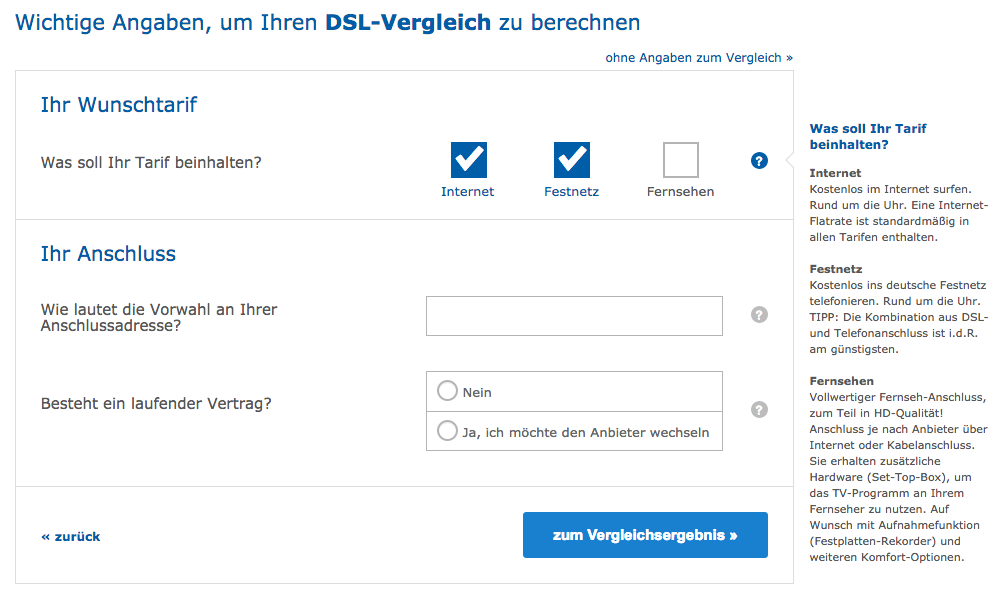
\includegraphics[width=0.8\textwidth]{images/ds-sys/check24_1}
	\caption{Check24.de asks for some data before the comparison of DSL contracts}
		\label{img:check24_1}
\end{figure}

\begin{figure}[tbp]
 \centering
	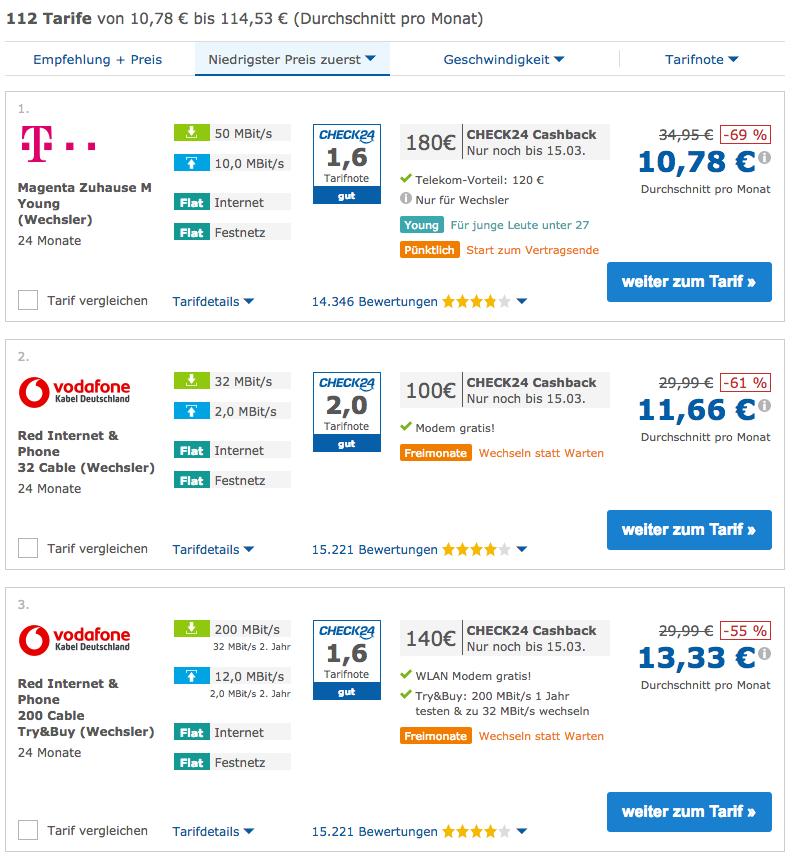
\includegraphics[width=0.8\textwidth]{images/ds-sys/check24_2}
	\caption{Check24.de DSL contract comparison result. The contracts can be sorted by domain-specific criterias.}
	\label{img:check24_2}
\end{figure}
The other sites work similar. All in all, they provide more of a ranking than a comparison.


Another interesting type of websites are Question Answering Portals like \emph{Quora.com}\footnote{\url{https://quora.com} (checked: 13.04.2018)} or \emph{GuteFrage.net}\footnote{\url{https://gutefrage.net} (checked: 13.04.2018)}. Although comparisons are not their primary goal, a lot of comparative questions are present on those sites.
On Quora, more than 2.380.000 questions have the phrase \enquote{better than} in their title. If \emph{Ruby} and \emph{Python} are added, 10.100 questions remain.\footnote{Checked via Google on 11.12.2017. Search phrase: \texttt{"better than" site:quora.com} and \texttt{ruby python "better than" site:quora.com}}
Same is true for the German site GuteFrage.net, though, the numbers are smaller than on Quora.com.\footnote{334.000 for \texttt{"besser als" site:gutefrage.net} and 78 for \texttt{ruby python "Besser als" site:gutefrage.net}}\newline

More interestingly are systems which can compare any objects on arbitrary properties, like \emph{Diffen.com}\footnote{\url{https://diffen.com} (checked: 13.04.2018)} and \emph{Versus.com}\footnote{\url{https://versus.com} (checked: 13.04.2018)}.

Versus.com aggregates freely available data sources like Wikipedia or official statistic reports. For example, the comparison of \enquote{Hamburg vs. Berlin} uses Wikipedia for the number of universities, \url{worldstadiums.com} for the availability of sport facilities and the Economist for the Big Mac Index. Presumably, human processing is involved as the possible comparisons are limited. For instance, a comparison of Hamburg and Darmstadt is not possible as Darmstadt is not available on Versus.com\footnote{Checked on 14.05.2018}. Likewise, \enquote{Ruby vs. Python} is not possible, Versus.com suggests to compare \enquote{Rome vs. Pyongyang} instead. Although Versus.com shows how many users \enquote{liked} the objects, it does not give a clear statement which one is better. For instance, it is not possible to check automatically whether Hamburg or Berlin is better for a short city trip. The user must manually search all valid properties like the number of museums, theaters, the price of public transport tickets and so on.

Similar to Versus.com, Diffen.com aggregates different data sources (see figures \ref{img:diffen} and \ref{img:versus}). All in all, the aggregated information is similar to Versus. The comparison is also tabular. Besides the automatically aggregated data, users can add information on their own. Diffen.com does not enforce any restrictions on the objects of comparison, but it faces the same problem as Versus as.com objects are missing. A comparison between Darmstadt and Hamburg is likewise not possible: all cells for Darmstadt in the table are empty.

\begin{figure}[htp]
 \centering
	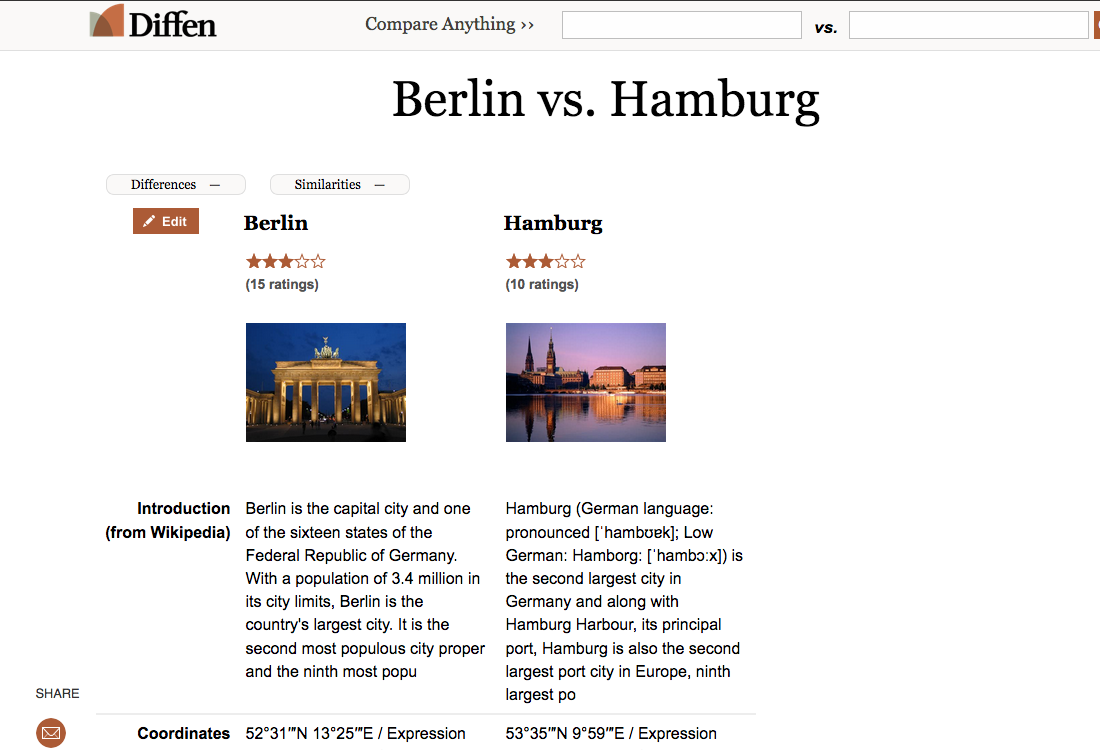
\includegraphics[width=0.8\textwidth]{images/ds-sys/diffen}
	\caption{The comparison of \enquote{Hamburg vs. Berlin} on Diffen.com}
		\label{img:diffen}
\end{figure}

\begin{figure}[htp]
    \centering
	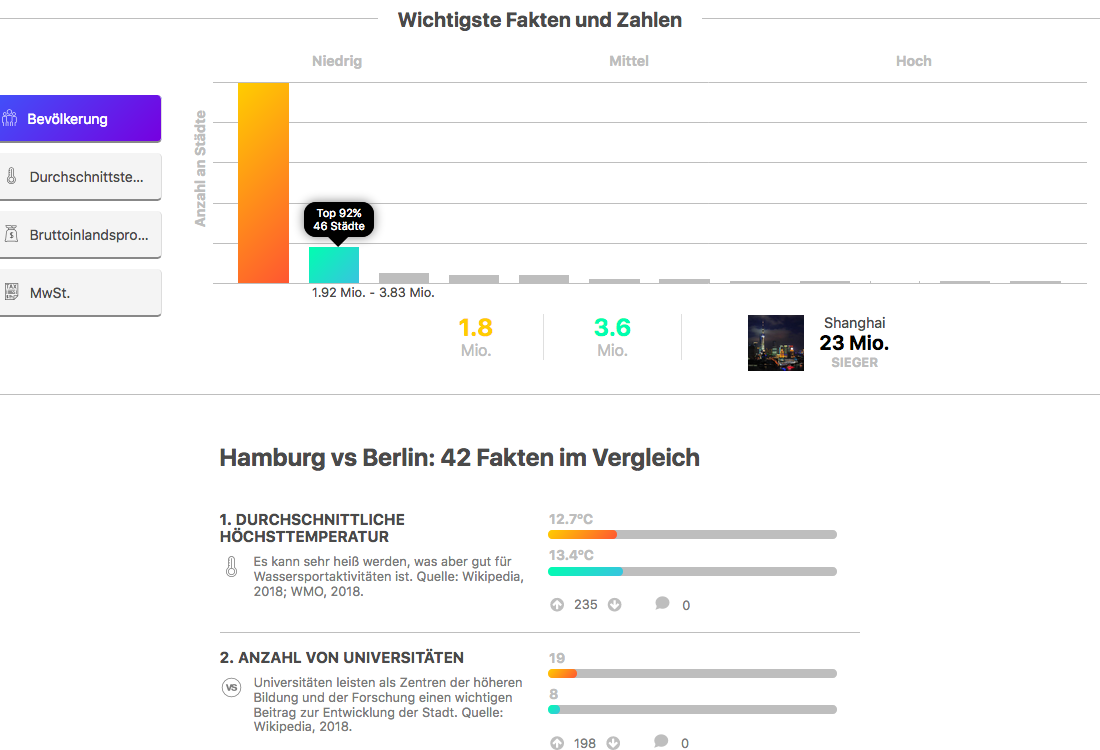
\includegraphics[width=0.8\textwidth]{images/ds-sys/versus}
	\caption{The comparison of \enquote{Hamburg vs. Berlin} on Versus.com}
		\label{img:versus}
\end{figure}

Neither Versus.com nor Diffen.com provides a comprehensible reason why an object is better than another one. They merely aggregate facts and bring them face to face. Despite the aggregation approach of both systems, many meaningful comparisons are not possible or not helpful (like \enquote{Hamburg vs. Darmstadt}, \enquote{Java vs. C\#}, \enquote{Dr Pepper vs. Orange Juice}).
Also, the user can not define the properties for the comparison. The sites provide every information available for the objects. For instance, Versus shows 42 properties for \enquote{Hamburg vs. Berlin} but only 35 for \enquote{Hamburg vs. Munich}.
\newline

To summarise, a lot of different comparison portals exist and are widely used. Especially the domain-specific portals do a good job, but inflexibility dearly buys the performance. First, the portals can only compare objects on predefined properties. Second, the data acquisition is not fully automatic. Domain-unspecific systems are good at aggregating information but do not provide a reasonable explanation to prefer X over Y.

Adding information like comments and product reviews can enrich the comparison with reasons and opinions, such as \enquote{Ruby is easier to learn than C} or \enquote{Python is more suitable for scientific applications than Erlang as many libraries exist}.

\FloatBarrier

\section{Machine Learning Methods}
\subsection{Recurrent Neural Networks and Long short-term memory}
A \emph{feed-forward (artificial) neural network (ANN)} can be seen as a directed, acyclic graph. The data flows sequentially from the input layer through the hidden layers until they reach the output layer. In contrast, \emph{recurrent neural networks (RNN)} can contain loops. The output of layer \emph{h} at time \emph{t} is part of the input of layer \emph{h} at time \emph{$t+1$}. In doing so, RNNs hold an internal state which is can be used to process sequential input like text\footnote{If a sentence is feed word by word into a ANN, each word is seen as an indepented data point. A RNN keeps the information about previous words.}. Figure \ref{fig:rnnschema} shows this idea.

\begin{figure}[ht]
\centering
	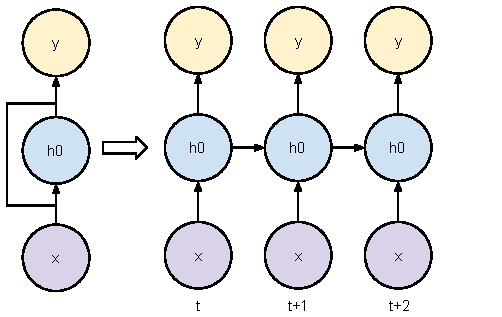
\includegraphics[width=0.9\textwidth,scale=0.5]{images/rnn_schema}
	\caption{Schematic view of an RNN. The right side shows the RNN unfolded for two time steps.}
		\label{fig:rnnschema}
\end{figure}

Different types of recurrent units have been used. A popular form are \emph{Long short-term memory (LSTM)} cells, as presented in \cite{hochreiter1997long}. LSTMs were developed to overcome the \emph{vanishing gradient problem}: gradients of early layers in deep networks tend to be small which makes the training difficult.


\subsection{Gradient Boosting}
The following overview is based on chapter ten of \cite{friedman2001elements}. Boosting is a technique to combine a set of weak learners into one good learner. The predicitions of a weak learner are only slightly better than random guessing.

The main idea behind \emph{gradient boosting} is to fit the weak learner sequentially on modified versions of the data, which creates the set of weak learners. In the end, the predictions of all weak learners \emph{$G_m$} are combined to produce the final prediction:

\[G(x) = \text{sign}\left(\sum^M_{m=1} \alpha_m G_m(x)\right) \]

The values for $\alpha_m$ are computed by the algorithm and determine how much the weak learner \emph{$G_m$} contributes to the prediction.

Boosting can be used with various machine learning algorithms and is suitable for regression as well as classification tasks. The boosting method used in this thesis is \emph{gradient boosting} with \emph{decision trees} as learners. In gradient boosting, \emph{$G_{m+1}$} is fitted on the residuals of \emph{$G_m$}. Thus, each tree tries to improve on the training examples on which the previous learner was weak on.

A frequently used implementation of gradient boosted decision trees is \emph{XGBoost}\footnote{\url{https://github.com/dmlc/xgboost} (checked 14.05.2018)}, as presentend in \cite{DBLP:journals/corr/ChenG16}.


\section{Performance measures}
Precision, Recall and f1 score are measures to check the classification performance. The measures are calculated per class.

The precision of a classifier with regards to class \emph{c} is defined as:
\[ \text{P(c)} = \frac{\text{\# of true positives}}{\text{\# true positives + \# false positives}} \]
Precision is the ratio between correctly predicted examples for class \emph{c} and all predicted examples of class \emph{c}.


The recall of a classifier with regards to class \emph{c} is defined as:
\[ \text{R(c)} = \frac{\text{\# of true positives}}{\text{\# true positives + \# false negatives}} \]


If only one out of 1000 examples was classified as \emph{c}, and the classification was correct, the precision for \emph{c} would be one, while the recall will be near zero. Likewise, if all  all examples are classified as \emph{c}, the recall will be one, while the precision will be zero. 

The f1 balances precision and recall. It is defined as the harmonic mean:
\[ F_{1}(c) = \frac{\text{2PR}}{\text{P+R}} \]

\section{Vector Representations for Documents}
% cosine similarity
Because many machine learning algorithms work with numeric values as input, text must be transformed into a numerical representation. Several methods are known to transform text into numeric feature vectors.
\subsection{Bag-of-words and bag-of-ngrams}
The \emph{bag-of-words} model is a simple vector representation for documents. All words in the corpus are collected into a vocabulary $\mathcal{V}$. A document j is representend by a vector $\vec{d_j}$ of size $|\mathcal{V}|$, where $\vec{d}_{j,i}$ is the frequency of word $\mathcal{V}_i$ in the document (the \emph{term frequency} $\text{tf}(i,j)$).

The model is fast to calculate but does not take any sequence or grammar information into accoun. It also ignores the significance of words. For instance, \enquote{\emph{the}} appears in almost every English text, while \emph{\enquote{psychology}} is seldom. Yet, this is not reflected in $\vec{d_j}$, as \enquote{\emph{the}} is likley to get a value as \emph{\enquote{psychology}}. Another problem is that the vectors are as long as the vocabulary (typically thousands of words) and sparse, which adds more parameters to learn.

The first problem can be reduced by using n-grams (hence, \emph{bag-of-ngrams}) instead of words. The vocabulary $\mathcal{V}$ will contain all sequences of \emph{n} consecutive words appearing in the corpus instead of single words. In this way, some sequence information is kept. The second problem can be solved by removing all very frequent words like \emph{\enquote{the}} or \emph{\enquote{can}} (often called stopwords) and by using a weighting function for the remaining words, most commonly \emph{term frequency, inverse document-frequency (tf-idf)}. With tf-idf, $\vec{d_{j,i}}$ is calculated as:

\[\vec{d_{j,i}} = \text{tf}_{i,j} \times \log{ \frac{N}{n_i} } \]

where \emph{N} is the total number of documents and $n_i$ is the number of documents the word (or n-gram) i appears in.

The other problems, sparsity and length, remain. They are solved in other vector representations.


\subsection{Mean Word Embeddings}
Word Embeddings are dense, low-dimension vector representations of words. They are learned by neural networks. The basic idea is to train an neural network on a suitable task. They weight matrix (\emph{embedding matrix}) of a defined hidden layer then contains the word embeddings.

The matrix is initialized with random values. After the network was trained, each column represents one word in $\mathcal{V}$ and each embedding has as many components as the hidden layer has neurons. This leads to word vectors which are much smaller than $|\mathcal{V}|$.

A method to learn word embeddings using a feed-forward neural network was presented in \cite{bengio2003neural}. The network was trained to predict the most likely next word given a number of preceding context words. This exploits the \emph{distributational hypothesis} (\cite{harris1954distributional}) which states that words which appear in similar contexts have a similar meaning. For instance, the network will see that the context \enquote{\emph{feed the}} is often followed by words like \enquote{\emph{cat}} or \enquote{\emph{dog}}, but never by \enquote{\emph{chair}}. In the end, the cosine similarity\footnote{a similarity metric for vectors: $\times$} between the learned vectors of related words (like cat and dog) is much higher than the cosine similarity between unrelated words (like cat and chair).

Two popular methods to learn word embeddings (extending the basic idea) are \emph{word2vec} (\cite{NIPS2013_5021}) and \emph{GloVe} (\cite{pennington2014glove}). In this thesis, \emph{GloVe} vectors are used, were each word is represented by a vector with 300 components.

The word embeddings can be used to create a dense, low-dimension vector representation for a document. This is done by taking the average of all word vectors in the document. In doing so, each sentence is represented by a \enquote{centroid word}. The efficiency of this method for several tasks is presented in \cite{Wieting:2015aa}.

\subsection{Sentence Embeddings and InferSent}
Bag-of-words an mean word embeddings lose sequence information. However, the sequence of words in a sentence is important for the meaning. For example, the sentence \enquote{\emph{I like cats, not dogs}} has a different meaning than \enquote{\emph{I like dogs, not cats}}, but both sentences will get the same bag-of-words vector and mean word embedding.

Sentence embeddings aim to learn embeddings for pieces of text instead of single words. In this way, sequence information is taken into account. Several methods have been proposed to create sentence embeddings (e.g. FastSent \cite{hill2016learning} and SkipTought \cite{NIPS2015_5950}). In this thesis, \emph{InferSent} as presented in \cite{Conneau:2017aa} is used.


InferSent learns sentence embedding in a similar way as word embeddings are learned. A neural network is trained on the \emph{Stanford Natural Language Inference (SNLI)} data set (\cite{snli:emnlp2015}). SNLI contains 570000 English sentence pairs. Each pair is labelled as \emph{entailment}, \emph{contradiction} or \emph{neutral}. Some examples are presented in table \ref{tbl:snli}. The authors assume that the \enquote{semantic nature} %zitat
makes the data set suitable for learning universal sentence embeddings.

\begin{table}[ht]
\caption{Example sentences from the \emph{Stanford Natural Language Inference (SNLI)} data set. Taken from \url{https://nlp.stanford.edu/projects/snli/} (checked: 14.05.2018)}
\label{tbl:snli}
\begin{tabularx}{\linewidth}{XXr}
\toprule
Premise & Hypothesis & Label \\ \midrule
A soccer game with multiple males playing. & Some men are playing a sport. & Entailment \\
A man inspects the uniform of a figure in some East Asian country. & The man is sleeping & Contradiction \\
A smiling costumed woman is holding an umbrella. & A happy woman in a fairy costume holds an umbrella. & Neutral \\
\bottomrule
\end{tabularx}
\end{table}


\begin{figure}[ht]
\centering
	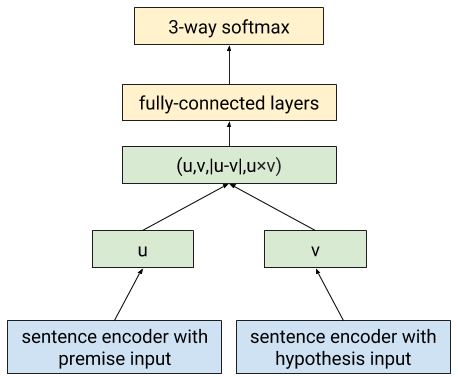
\includegraphics[width=0.5\textwidth,scale=0.5]{images/nli}
	\caption{Generic training scheme of \emph{InferSent}. Six \emph{sentence encoder} variants were tested.  (Adapted from \cite{Conneau:2017aa})}
		\label{fig:infersent}
\end{figure}


The architecture of the neural network is presented in figure \ref{fig:infersent}. Two separate encoders are used to encode the text and the hypothesis. The embeddings \emph{u} and \emph{v} are combined into a feature vector which contains the concatenation, the element-wise product and the element-wise difference of \emph{u} and \emph{v}. This vector, containing information from both sentences, is then fed into a fully connected layer and a softmax layer which outputs the probabilities of each label.

The authors tested six architectures for the sentence encoder: LSTM (\cite{hochreiter1997long}), GRU (\cite{cho2014properties}), BiLSTM with mean/max pooling (\cite{collobert2008unified}), self-attentive networks (\cite{liu2016learning}, \cite{lin2017structured}) and hierarchical ConvNet (\cite{zhao2015self}). 

Twelve transfer task\footnote{For example: binary classification (sentiment analysis, product reviews, subjectivity/objectivity, opinion polarity), multi-class classification (question type), entailment and semantic relatedness, semantic tectual similarity, paraphrase detection and caption-image retrieval.} were used to test the quality of the embeddings. For each task and encoder architecture, the embeddings were used as features. Logistic Regression was used as the machine learning algorithm.

The embeddings generated by the BiLSTM with max pooling and an embedding size of 4096 yielded the best accuracy for SNLI and the transfer tasks. Also, the embeddings were better than other state-of-the-art sentence embeddings like SkipThought.

A pretrained model for InferSent is available on GitHub\footnote{\url{https://github.com/facebookresearch/InferSent} (checked 13.05.2018)}. This model is used in section \ref{sec:features}.

\subsection{HypeNet and LexNet}
\label{sec:lexnet}
HypeNet, presented in \cite{DBLP:conf/acl/ShwartzGD16}, is a method to detect hypernym relations between words. It combines distributational and dependency path based methods to create a vector representation for word pairs. LexNet, presented in \cite{DBLP:journals/corr/ShwartzD16}, is a generalisation of HypeNet, which is able to detect multiple semantic relationships between two words.

The dependency paths add information about joint occurences of the two words, while the distributational methods add information about the terms in separate contexts. Word Embeddings are used as distributational features.

For each term pair, all dependency paths were extracted. Each edge was represented as \texttt{lemma/POS/dependency label/direction}. An example is given in figure \ref{fig:hypenet}. 

\begin{figure}[h]
\centering
\caption{Dependency parse of the example sentence \emph{parrot is a bird}, where the relationship between parrot and bird is of interest. This path is represented as \texttt{X/NOUN/nsubj/< be/VERB/ROOT/- Y/NOUN/attr/>} (Adapted from \cite{DBLP:conf/acl/ShwartzGD16}).}
\label{fig:hypenet}
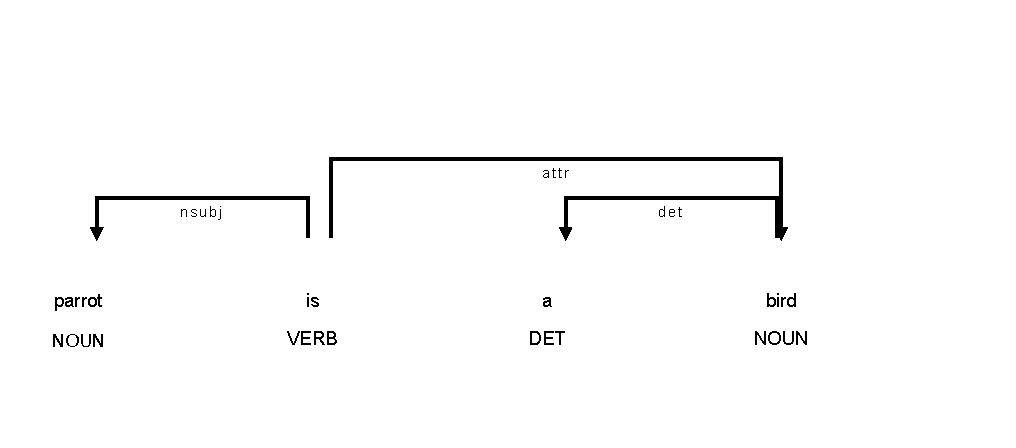
\includegraphics{images/hypenet_example}
\end{figure}


The paths were encoded using an LSTM. The average of all encoded paths was then used as the path information for the word pair. The combination of distributational and path information outperformed state-of-the-art techniques.\newline

The task at hand is different from the detection of semantic relations. The relation of two nouns\footnote{The situation might be different if proper nouns are also used. Fruit is an hypernym for apple, but not for the company Apple.} with respect to hypernymy is unambigous. Bird is a hypernym for parrot in all cases. Yet the task is not to search for hypernyms or any other semantic relation. It is not possible to assign the correct class by only looking at the objects. For example, there might be sentences saying that \emph{Python} is better than \emph{Ruby}, while others say it is not.

However, it is expected that the dependency path between the objects of interest adds valuable information. This thesis reuses the idea on how to extract and encode paths between two words.




\chapter{Building a data set for Comparative Argument Mining}
There's not dataset.
\section{Common Crawl Text Corpus}
The raw data used for the creation of the dataset was derived from CommonCrawl. CommonCrawl is a non-profit organisation which crawls the web and releases the data and metadata with a loose license. This master thesis uses the crawl data from DATE. Furthermore, the data was processed: HTML was stripped out, and the content was splitted into sentences using X. To make the data maintainable, the sentences where imported into an ElasticSearch index. The index has a size of 1.1tb and contains 3,288,963,864 unique sentences.

To get an idea how many sentences in the index may be comparative, searches with cue words was performed. The query \ref{lst:es-cc-query} yields 55,627,400 results, the more specific query \texttt{is better than} yields 428,932 results.

\begin{lstlisting}[label=lst:es-cc-query,breaklines=true,postbreak=\mbox{\textcolor{red}{$\hookrightarrow$}\space},caption=Candidates for Comparative Sentences]
{
  "query":{
    "bool":{
      "must":[
        {
          "query_string":{
            "default_field":"text",
            "query":"better OR easier OR faster OR nicer OR wiser OR cooler OR decent OR safer OR superior OR solid OR teriffic OR worse OR harder OR slower OR poorly OR uglier OR poorer OR lousy OR nastier OR inferior OR mediocre"
          }
        }
      ]
    }
  }
}
\end{lstlisting}

Those numbers indicate that the index contains enough comparative sentences to create machine learning data set.

Lesen \cite{Panchenko:2017aa}

\section{Prestudy}
Previous to the main study, a pre-study was conducted to assess the quality of the annotation guidelines, the approach of sentence generation and the task itself.


\subsection{Data Selection and Preprocessing}
\label{sec:prestudy-processing}
To obtain comparative sentences from the ElasticSearch index, Query \ref{lst:es-query-a} was used. The sentence must contain two comparable objects (like "Apple" and "Pear") and at least one cue word. Presence of the cue words \enquote{better}, \enquote{worse}, \enquote{superior} and \enquote{inferior} should increase the probability of the sentence to be comparative. In this way, the amount of noisy sentences should be reduced.
However, not all comparisons will contain one of the cue words, so 25\% of the sentences sentences where obtained without the cue words.


\begin{lstlisting}[label=lst:es-query-a,breaklines=true,postbreak=\mbox{\textcolor{red}{$\hookrightarrow$}\space},caption=Prestudy Sentence Selection Query]
{
  "query":{
    "bool":{
      "must":[
        {
          "query_string":{
            "default_field":"text",
            "query":"(better OR worse OR superior OR inferior) AND \"<OBJECT_A>\" AND \"<OBJECT_B>\""
          }
        }
      ]
    }
  }
}
\end{lstlisting}



Ten hand-selected object pairs were used (see table \ref{tbl:prestudy-objects}). It was expected that those pairs will yield differently phrased comparisons, as, for instance, cars are compared in a different way than programming languages. Some sentences contain programming- and computer specific terms, so a need for this knowledge was expressed in the title of the crowdsourcing task.
\begin{table}[h]
\centering
\caption{Objects of the Annotation Prestudy}
\label{tbl:prestudy-objects}
\begin{tabular}{@{}llrrr@{}}
\toprule
First Object & Second Object      & \# Sentences                             \\ \midrule
Ruby    & Python    & 109      \\
BMW    & Mercedes    & 107  \\
USA & Europe & 106 \\
Beef & Chicken & 106   \\
Android & iPhone    &   104  \\
Cat & Dog      &     104  \\ 
Football & Baseball   &  104 \\ 
Wine & Beer  & 104  \\
Car & Bicycle & 103 \\
Summer & Winter &  103\\  \midrule 
 & & 1050 \\ 
\bottomrule  
                               
\end{tabular}
\end{table}

All retrieved sentences contain each of the objects exactly once.

\subsection{Task}
Using the method described above, 1050 sentences were obtained for the prestudy. The annotators were asked to assigne one of the following classes to the sentences. Each sentence was annotated by three annotators.

The annotators where asked to assign one of the four classes (see table \ref{tbl:prestudyclasses}) to each sentence.

\begin{table}[h]
\centering
\caption{Classes for the Prestudy}
\label{tbl:prestudyclasses}
\begin{tabular}{@{}ll@{}}
\toprule
Class & Description \\ \midrule
BETTER & The first object in the sentence (object A) is better than the second one (object B)\\
WORSE & The first object is worse \\
UNCLEAR & Neither BETTER nor WORSE fits, but the sentence is comparative\\
NO\_COMP & The sentence is not comparative\\
\bottomrule
\end{tabular}
\end{table}



In a first step, 100 sentences were annotated. To ensure the quality, twelve additional sentences were setup as test sentences. If one annotator failed three test sentences, he was removed from the task.

The sentences were preprocessed: the first object was replaced by OBJECT\_A, the second by OBJECT\_B. Examples are shown in table \ref{tbl:pre1s}. The removal was done so that the annotators can concentrate on the comparative structure of the sentence and are not biased by the objects.


% Beispielsätze PreStudy 1. Teil
\begin{table}[h]
\centering
\caption{Sentences for the first step}
\label{tbl:pre1s}
\begin{tabular}{{p{12cm}p{3cm}}}
\toprule
Sentence            & Expected Class \\ \midrule
This is potentially useful for OBJECT\_A, PHP, JS and OBJECT\_B.                                 & NO\_COMP       \\
Also keep in mind that OBJECT\_A blends will give you worse mileage than OBJECT\_B & WORSE      \\ 
Snowboarding during OBJECT\_A is a lot better than during OBJECT\_B. & BETTER \\
\bottomrule
\end{tabular}
\end{table}



This test step delivered valuable insights. First, the amount of test sentences was to small. Users might see the same test sentence twice. Second, the phrasing of the annotation guidelines was to confusing, especially the distinction between NO\_COMP and UNCLEAR as well as their class names.
Third, the complete removal of the original objects is suspected to partly obscure the sense of the sentences.\newline

In a second step, 200 new sentences were annotated, again with three annotations per sentences. This time, 51 test questions were used, so that it is less likely that annotators will see the same question twice. Furthermore, the preprocessing was changed. Instead of removing the original objects, :[OBJECT\_A] was appended to the first object, :[OBJECT\_B] to the second object. Also, each object was highlighted in a different color. Example sentences are shown in table \ref{tbl:pre2s}. In this way, the annotators could quickly see the objects of interest while the sense of the sentence remains intact.
% Beispielsätze PreStudy 2. Teil
\begin{table}[h]
\centering
\caption{Sentences for the second step}
\label{tbl:pre2s}
\begin{tabular}{{p{12cm}p{3cm}}}
\toprule
Sentence                                                                                                           & Expected Class \\ \midrule
I'd go with \textbf{{\color[HTML]{9A14B2} python:{[}OBJECT\_A{]}}} or \textbf{{\color[HTML]{6CB219}ruby:{[}OBJECT\_B{]}}}.                                 & NO\_COMP       \\
I prefer \textbf{{\color[HTML]{9A14B2}ruby:{[}OBJECT\_A{]}}} over \textbf{{\color[HTML]{6CB219}python:{[}OBJECT\_B{]}}} on windows.                                              & BETTER         \\
I've tried \textbf{{\color[HTML]{9A14B2}python:{[}OBJECT\_A{]}}}, and can see why people like it, but \textbf{{\color[HTML]{6CB219}ruby:{[}OBJECT\_B{]}}} suits my style better. & WORSE          \\
i think this car is a far better deal than the \textbf{{\color[HTML]{9A14B2}bmw{:[OBJECT\_A]}}} 5 series or \textbf{{\color[HTML]{6CB219}mercedes:[OBJECT\_B]}} 320e.                                                                                                                &        UNCLEAR        \\ \bottomrule
\end{tabular}
\end{table}

\label{sec:annotation-guidelines}
\subsection{Results}
Each sentence was annotated by three annotators. Figure \ref{pre:dist} shows the class distribution.

\begin{figure}[h]
\centering
\caption{Class Distribution in the prestudy}
\label{pre:dist}
\begin{tikzpicture}
\pie [rotate=180, text = legend, color= {cgray, cgreen, cred, cblue}]
    {59.76/NO\_COMP (150),
    23.11/BETTER (58),
    9.16/WORSE (23),
    7.97/UNCLEAR (20)}
\end{tikzpicture}
\end{figure}


%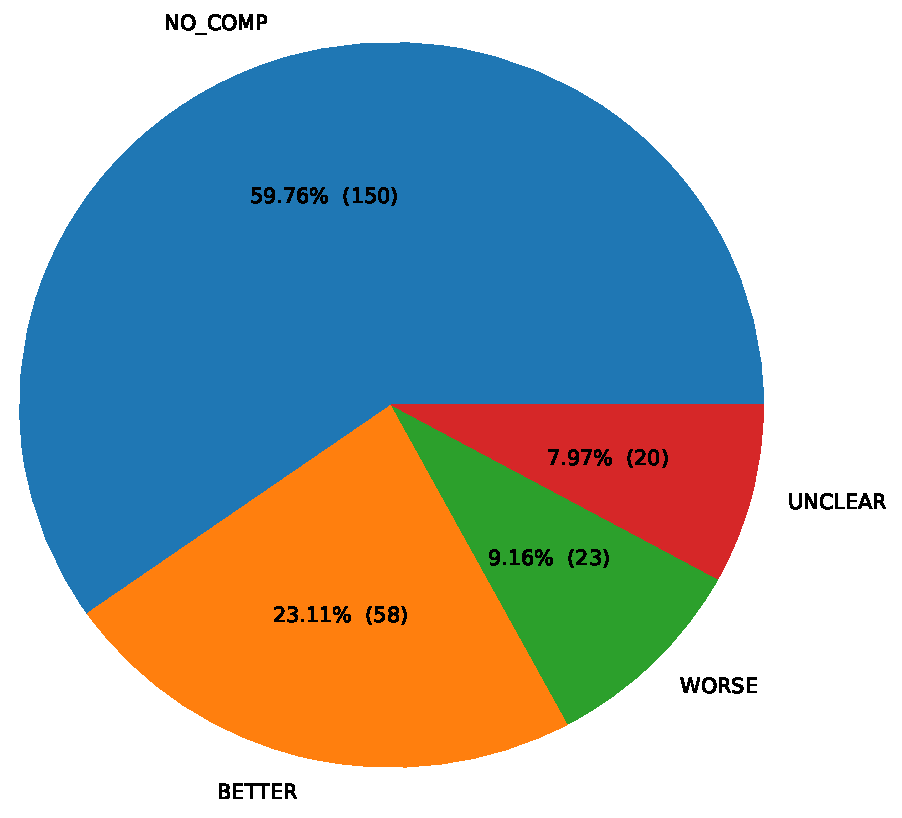
\includegraphics[scale=0.6]{images/prestudy/label_distribution.pdf}


Crowdflower has a trust value for each annotator. This trust value and the number of votes per class gives a value of confidence for each label.\footnote{How the confidence is calculated in detail can be found at https://success.crowdflower.com/hc/en-us/articles/201855939-How-to-Calculate-a-Confidence-Score (Last checked: 19.12.2017)}


As presented in figure \ref{pre:conf}, a majority (151) of the labelings has a confidence greater or equal to 0.9, and 15 sentences a confidence below 0.6; the mean is 0.86. Detailed numbers on the confidence are shown in table \ref{pre:conf-table}

\begin{figure}
\centering
\caption{Confidence histogram}
\label{pre:conf}
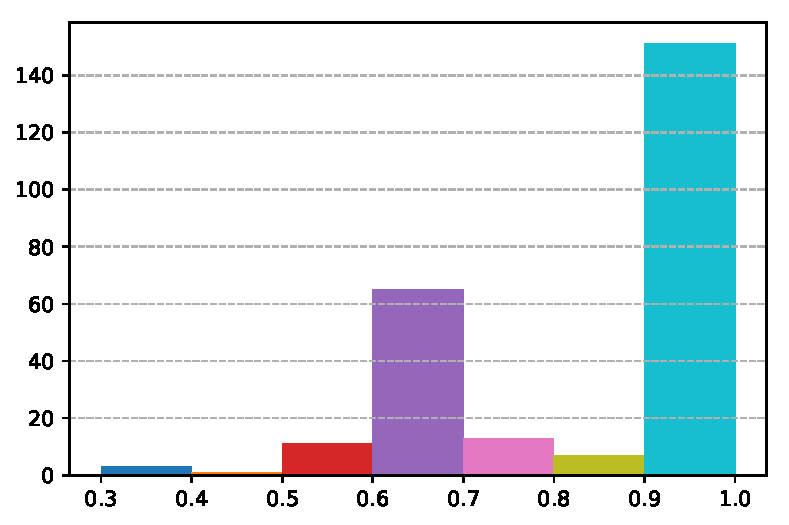
\includegraphics[scale=0.6]{images/prestudy/confidence.pdf}
\end{figure}


\begin{figure}[h]
\centering
\caption{Confidence}
\begin{tabular}{@{}ll@{}}
\toprule
Type & Value  \\ \midrule
Average Confidence & 0.86 \\
Standard Derivation & 0.17 \\
Lowest Confidence & 0.35\\
Highest Confidence & 1.00\\
25th percentile average & 0.67\\
50th percentile average & 1.00\\
\bottomrule
\label{pre:conf-table}
\end{tabular}
\end{figure}





The most difficult sentence is with a confidence of 0.35 for the class \emph{WORSE} was
\begin{quote}
Google shouldn't have mandated an inferior map app on the iphone:[OBJECT\_A] (as opposed to android:[OBJECT\_B]).
\end{quote}

It was labelled as \emph{BETTER} (trust: 0.72), \emph{WORSE} (trust: 0.85) and \emph{NO\_COMP} (trust: 0.82). The class \emph{WRONG} is correct here, as the object \enquote{iphone} is inferior to \enquote{android} on the aspect of \enquote{map app}.

The following sentence was assigned to \emph{BETTER} (0.37 confidence), although it should belong to \emph{UNCLEAR}.
\begin{quote}
Not to mention that the iphone:[OBJECT\_A] and android:[OBJECT\_B] phones deliver a far superior user experience overall
\end{quote}
However, the annotator for \emph{UNCLEAR} only had 0.87 trust, while the one for \emph{BETTER} had 1 (third one was \emph{NO\_COMP} with 0.82 trust).\newline

All things considered, the result of the prestudy is satisfactory. The annotators agreed in the majority of decisions. 


\newpage
\section{Main Study}
\subsection{Task Description}
\subsection{Data Generation}
Three domains were fixed for the sentences of the main study. The domains were chosen in a way that a majority of people can decide whether a sentence contains a comparison or not.

The most specific domain was "Computer Science Concepts". It contains objects like programming languages, database products and technology standards such as Bluetooth and Ethernet.  Many computer science concepts can be compared objectively, for instance, one can compare Bluetooth and Ethernet on their transmission speed. Some basic knowledge of computer science was needed to label sentences correctly. For example, to compare Eclipse and NetBeans, the annotator must know what an Integrated Development Environment (IDE) is and that both objects are Java IDEs.  The need of the knowledge was communicated to the prospective annotators. The objects for this domain were manually extracted from "List of ..." articles from Wikipedia.

The second, broader domain was "Brands". It contains objects from of different types (car brands, electronics brands, and food). As brands are present in everyday life of people, it is expected that anyone can label the majority of sentences containing well known brands such as Coca-Cola or Mercedes. As with computer science, the objects for this domain were extracted from "List of ..." articles from Wikipedia.

The last domain is not restricted to any topic. For each one of 25 randomly selected seed words, ten similar words were extracted using JoBimText, a software package for distributional semantics. The seed words were created using https://randomlists.com\footnote{Last checked: 25.01.2018}. Listing \ref{lst:jbtres} shows the result\footnote{http://ltmaggie.informatik.uni-hamburg.de/jobimviz/ws/api/stanford/jo/similar/harvard\%23NP?numberOfEntries=10&format=json Last checked: 25.01.2018; Some uninteresting fields were removed for brevity} for the seed word \emph{harvard}.

\begin{lstlisting}[language=json,label=lst:jbtres,caption=Similar words to "Harvard"]
{
   "results":[
      { "score":688.0, "key":"harvard#NP" },
      { "score":245.0, "key":"yale#NP" },
      { "score":163.0, "key":"princeton#NP" },
      { "score":152.0, "key":"mit#NP" },
      { "score":143.0, "key":"stanford#NP" },
      { "score":133.0, "key":"university#NP"},
      { "score":132.0, "key":"tufts#NP" },
      { "score":130.0,"key":"cornell#NP"},
      { "score":127.0, "key":"nyu#NP" },
      { "score":113.0, "key":"university#NN" }
   ]
}
\end{lstlisting}
This method covers a wide are of possible comparison patterns.\newline

Especially for brands and computer science, the object lists are long (4493 brands and 1339 for computer science).The frequency of each object was checked using a frequency dictionary to reduce the number of possible pairs. All objects with a frequency of zero and ambiguous objects were removed from the list. For instance, the objects "RAID" (a hardware concept) and "Unity" (a game engine) were removed from the computer science list as they are also regularly used nouns.

The remaining objects were combined to pairs. For each type, all possible combinations were created. For brands and computer science, the type is the source list. For the unrestricted domain, the seed word was used. This procedure guarantees that only meaningful pairs are created.
The ElasticSearch Index was then queried for entries containing both objects of each pair. For 90\% of the queries, the marker terms where added to the query. This was done to check whether there is a chance that those two objects were compared. All pairs were the query yielded at least 100 sentences were kept. Those pairs are frequent enough and have a high chance of generating comparative sentences.

From the sentences of those pairs, 2500 for each category were randomly sampled as candidates for the crowdsourcing campaign. 250 sentences were manually labelled to check if there are enough comparative sentences. Those labels were discarded for the crowdsourcing campaign.
The label distribution of the 250 sentences is presented in the figures FIGURE NUMBERS.

\begin{figure}[h]
    \centering
    \begin{minipage}{0.49\textwidth}
        \centering
       \begin{tikzpicture}
\pie [rotate=180,radius=2,color= {cgray, cgreen, cred, cblue}]
    {68.9/NONE,
    15.2/BETTER,
    5.7/WORSE,
    10.2/OTHER }
    \label{pre:brands}
\end{tikzpicture}        \caption{Brands}
    \end{minipage}\hfill
    \begin{minipage}{0.49\textwidth}
        \centering
      \begin{tikzpicture}
\pie [rotate=180,radius=2, color= {cgray, cgreen, cred, cblue}]
    {53.00/NONE,
    19.70/BETTER,
    11.60/WORSE,
    15.70/OTHER }
\end{tikzpicture}
        \caption{Computer Science}
    \end{minipage}
    \end{figure}
    
    \begin{figure}[h]
    \centering
    \begin{minipage}{0.49\textwidth}
        \centering
       \begin{tikzpicture}
\pie [rotate=180,radius=2,color= {cgray, cgreen, cred, cblue}]
    {65.50/NONE,
    16.10/BETTER,
    7.20/WORSE,
    11.20/OTHER }
\end{tikzpicture}        \caption{Unrestricted}
    \end{minipage}\hfill
    \end{figure}
    
In all samples, at least 30\% of the sentences are comparative. This number shows that the sampling method is sufficient to sample sentences for the crowdsourcing campaign.

\chapter{Classification of Comparative Sentences}
The data collected from the crowdsourcing task was used as training data for two classification problems. In the first problem, a machine learning algorithm was trained to predict one of the three classes per sentence (see table \ref{tbl:mainstudy-classes}). The second problem is a simplification of the first one as it is designed as a binary classification problem. The classes \texttt{BETTER} and \texttt{WORSE} were merged into the class \texttt{ARG}.

The data was split into a training set (5820 sentences; 4240 \texttt{NONE}, 1102 \texttt{BETTER} and 478 \texttt{WORSE}) and a held-out set.
The experiments were conducted on the training set only. During the development, the experiments were evaluated using stratified k-fold cross-validation where k equals five. 

The held-out set stayed untouched until the final evaluation presented in section \ref{sec:final}.

If not stated otherwise, scikit-learn (\cite{scikit-learn}) was used to perform feature processing, the classification and evaluation.

\section{Choice of Algorithms}
\begin{table}[!h]
\centering

\caption{Tested classification algorithms. Precision, recall and f1 score are calculated as weighted macro-average across classes (as in scikit-learn's \texttt{classification\_report}). The best out of five folds with standard derivation in brackets is presented.}
\label{tbl:algo}
\begin{tabularx}{\textwidth}{Xrrr}
\toprule
Algorithm & Precison & Recall & F1 Score \\ \midrule
\textbf{XGBClassifier} 	&	 \textbf{0.79} \scriptsize{(0.01)} &  \textbf{0.81} \scriptsize{(0.01)} &  \textbf{0.78} \scriptsize{(0.01)}  \\

Logistic Regression 	&	 0.77 \scriptsize{(0.01)} &	 0.79 \scriptsize{(0.01)} &	 0.78 \scriptsize{(0.01)}  \\ 


Stochastic Gradient Descent 	&	 0.76 \scriptsize{(0.01)} &	 0.77 \scriptsize{(0.01)} &	 0.77 \scriptsize{(0.01)}  \\ 

Ada Boost (Decision Trees) 	&	 0.75 \scriptsize{(0.01)} &	 0.78 \scriptsize{(0.00)} &	 0.75 \scriptsize{(0.01)}  \\ 

Support Vector Machine (Linear Kernel) &	 0.76 \scriptsize{(0.01)} &	 0.75 \scriptsize{(0.01)} &	 0.75 \scriptsize{(0.01)}  \\ 


K Neighbors (k = 5) &	 0.77 \scriptsize{(0.03)} &	 0.78 \scriptsize{(0.01)} &	 0.75 \scriptsize{(0.01)}  \\ 


Random Forest &	 0.76 \scriptsize{(0.01)} &	 0.78 \scriptsize{(0.00)} &	 0.75 \scriptsize{(0.01)}  \\ 

Decision Tree &	 0.74 \scriptsize{(0.01)} &	 0.75 \scriptsize{(0.01)} &	 0.74 \scriptsize{(0.01)}  \\ 

Extra Trees 	&	 0.74 \scriptsize{(0.01)} &	 0.78 \scriptsize{(0.00)} &	 0.74 \scriptsize{(0.00)}  \\ 

Multinomial Gaussian Bayes &	 0.69 \scriptsize{(0.04)} &	 0.77 \scriptsize{(0.01)} &	 0.71 \scriptsize{(0.01)}  \\ 


Support Vector Machine (RBF Kernel) 	&	 0.53 \scriptsize{(0.00)} &	 0.73 \scriptsize{(0.00)} &	 0.61 \scriptsize{(0.00)}  \\ 

Support Vector Machine (Polynomial Kernel) 	&	 0.53 \scriptsize{(0.00)} &	 0.73 \scriptsize{(0.00)} &	 0.61 \scriptsize{(0.00)}  \\

Support Vector Machine (Sigmoid Kernel) &	 0.53 \scriptsize{(0.00)} &	 0.73 \scriptsize{(0.00)} &	 0.61 \scriptsize{(0.00)}  \\ 


\bottomrule
\end{tabularx}
\end{table}

To find the best performing classification algorithms, thirten (see table \ref{tbl:algo}) were selected and compared. Except \emph{XGBoost}\footnote{XGBoost is not part of scikit-learn. The implementation presented in \cite{DBLP:journals/corr/ChenG16} was used.} and \emph{Extra Trees Classifier}, all algorithms were used in at least one paper presented in section \ref{sec:argmine}. The binary unigram vector computed on the whole sentence was used as the only feature. Stratified k-fold with k equals five was used to assess the quality of the algorithm.





%\begin{table}[h]
%\centering
%\label{tbl:algo}
%\caption{All evaluated classification algorithms. The F1 score shows the classification performance with the unigram feature.}
%\begin{tabularx}{\textwidth}{XlX}
%\toprule
%Algorithm & F1 Score & Used in\\ \midrule
%
%XGBoost & 0.76 & -\\ 
%
%Logistic Regression & 0.75 &  \cite{Dusmanu2017Argument-Mining,Daxenberger2017What-is-the-EssAker2017What-works-and-,Lippi2016Argumentation-M}\\ 
%
%AdaBoost & 0.74 &  \cite{Aker2017What-works-and-}\\  
%
%Linear SVC & 0.73 & \cite{Aker2017What-works-and-}\\  
%
%Decision Tree & 0.72 &  \cite{Stab2014Identifying-Arg,Lippi2016Argumentation-M}\\ 
%
%Stochastic Gradient Descent & 0.72 & -\\ 
%
%
%Random Forest & 0.72 &  \cite{Dusmanu2017Argument-Mining,Stab2014Identifying-Arg,Eckle-Kohler2015On-the-Role-of-,Aker2017What-works-and-,Lippi2016Argumentation-M}\\  
%
%Extra Trees Classifier & 0.72 & - \\
%
%K Neighbors & 0.72 &  \cite{Aker2017What-works-and-}\\ 
%
%
%Support Vector Machine (non-linear kernel) & 0.60 & \cite{Stab2014Identifying-Arg,Eckle-Kohler2015On-the-Role-of-,Park:2012:ICC:2391171.2391173,Lippi2016Argumentation-M,Habernal2016Argumentation-M}\\ 
%
%
%Naive Bayes & 0.60 & \cite{Stab2014Identifying-Arg,Eckle-Kohler2015On-the-Role-of-,Aker2017What-works-and-,Park:2012:ICC:2391171.2391173,Lippi2016Argumentation-M}\\  
%
%
% \bottomrule 
%\end{tabularx}
%
%\end{table}


Tree-based methods and linear models work good. Support Vector Machines with non-linear kernels assigne \texttt{NONE} to all sentences.

As XGBoost and Logistic Regression already work in a pleasing way, no further investigations on the performance of other algorithms were done. A set of hyper-parameters for XGBoost were tested using exhaustive grid search and randomized search. However, no significant increase in the F1 score could be achieved.

In the following sections, all experiments were done using XGBoost.


\section{Preprocessing}
In addition to the full sentence, preprocessed versions of it were used in the feature calculation.

Different parts of the sentence were used. The \emph{first part} contains all words from the beginning of the sentence to the first object, while the \emph{last part} contains all words from the second object to the end of the sentence. The \emph{middle part} contains all words between the first and the second object.

Another processing step was done to assess how important the objects are for the classification. The objects either stayed untouched, were removed or replaced. Two different replacement strategies were tested. First, both objects were replaced by the term \emph{OBJECT} (replacement). Second, the first object was replaced by \emph{OBJECT\_A} and the second by \emph{OBJECT\_B} (distinct replacement). Some examples are shown in table \ref{preprocessing_example}.

\begin{table}[h]
\centering

\caption{Preprocessing examples for the sentence \enquote{\emph{In my mind, Python is better than Ruby}}}
\label{preprocessing_example}
\begin{tabularx}{\linewidth}{lX}
\toprule
Preprocessing & Result \\ \midrule
Middle part & Python is better than Ruby \\
Middle part, removal & is better than \\
Full sentence, distinct replacement &In my mind, OBJECT\_A is better than OBJECT\_B \\
First part, removal & In my mind, \\
\bottomrule
\end{tabularx}

\end{table}


\section{Features}

\section{Baselines}
\label{sec:3_baseline}
As described in section \ref{sec:argmine}, there is no task which is similar enough to this one which could be used as a baseline. Thus, two baselines using the obtained data were created. The first baseline, shown in table \ref{tbl:3stratifiedbaseline}, assigns all sentences to the class \texttt{NONE}.

% 24.3
\begin{table}[!htb]
    \begin{minipage}{.5\linewidth}
      \caption{Random (stratified) baseline for the classification task.}
      \label{tbl:3stratifiedbaseline}
      \centering
      
\begin{tabular}{@{}lrrrr@{}}
\toprule
 	&	 precision &	 recall &	 f1 score  \\ \midrule 
\texttt{BETTER}	&	 0.22 \scriptsize{(0.02)} &	 0.23 \scriptsize{(0.02)} &	 0.22 \scriptsize{(0.02)}  \\ 
\texttt{WORSE}	&	 0.10 \scriptsize{(0.02)} &	 0.08 \scriptsize{(0.02)} &	 0.09 \scriptsize{(0.02)}  \\ 
\texttt{NONE}	&	 0.74 \scriptsize{(0.01)} &	 0.74 \scriptsize{(0.01)} &	 0.74 \scriptsize{(0.01)}  \\ 
average	&	 0.59 \scriptsize{(0.01)} &	 0.59 \scriptsize{(0.01)} &	 0.59 \scriptsize{(0.01)}  \\ 
\bottomrule
\end{tabular} 

  \end{minipage}%
    \begin{minipage}{.5\linewidth}
      \centering
        \caption{Majority class baseline for the classification task.}
        \label{tbl:3majoritybaseline}
\begin{tabular}{@{}lrrrr@{}}
\toprule
 	&	 precision &	 recall &	 f1 score  \\ \midrule 
\texttt{BETTER}	&	 0.00 \scriptsize{(0.00)} &	 0.00 \scriptsize{(0.00)} &	 0.00 \scriptsize{(0.00)}  \\ 
\texttt{WORSE}	&	 0.00 \scriptsize{(0.00)} &	 0.00 \scriptsize{(0.00)} &	 0.00 \scriptsize{(0.00)}  \\ 
\texttt{NONE}	&	 0.73 \scriptsize{(0.00)} &	 1.00 \scriptsize{(0.00)} &	 0.84 \scriptsize{(0.00)}  \\ 
average	&	 0.53 \scriptsize{(0.00)} &	 0.73 \scriptsize{(0.00)} &	 \textbf{0.61} \scriptsize{(0.00)}  \\ 
\bottomrule
\end{tabular}
    \end{minipage} 
\end{table}



The second baseline is created by assigning classes to the data at random, respecting the distribution of classes in the original data. The results are shown in table \ref{tbl:3majoritybaseline}.

% 24.3
The baselines for the binary classification task are shown in tables \ref{tbl:binmaj} and \ref{tbl:binstrat}.


\begin{table}[!htb]
    \begin{minipage}{.5\linewidth}
      \caption{Random (stratified) baseline for the binary classification task.}
      \label{tbl:binmaj}
      \centering
      
\begin{tabular}{@{}lrrrr@{}}
\toprule
 	&	 precision &	 recall &	 f1 score  \\ \midrule 
\texttt{ARG}	&	 0.31 \scriptsize{(0.02)} &	 0.31 \scriptsize{(0.02)} &	 0.31 \scriptsize{(0.02)}  \\ 
\texttt{NONE}	&	 0.74 \scriptsize{(0.01)} &	 0.74 \scriptsize{(0.01)} &	 0.74 \scriptsize{(0.01)}  \\ 
average	&	 0.62 \scriptsize{(0.01)} &	 0.62 \scriptsize{(0.01)} &	 \textbf{0.62} \scriptsize{(0.01)}  \\ 
\bottomrule
\end{tabular}

  \end{minipage}%
    \begin{minipage}{.5\linewidth}
      \centering
        \caption{Majority class baseline for the binary classification task.}
        \label{tbl:binstrat}
\begin{tabular}{@{}lrrrr@{}}
\toprule
 	&	 precision &	 recall &	 f1 score  \\ \midrule 
\texttt{ARG}	&	 0.00 \scriptsize{(0.00)} &	 0.00 \scriptsize{(0.00)} &	 0.00 \scriptsize{(0.00)}  \\ 
\texttt{NONE}	&	 0.73 \scriptsize{(0.00)} &	 1.00 \scriptsize{(0.00)} &	 0.84 \scriptsize{(0.00)}  \\ 
average	&	 0.53 \scriptsize{(0.00)} &	 0.73 \scriptsize{(0.00)} &	 0.61 \scriptsize{(0.00)}  \\ 
\bottomrule
\end{tabular}
    \end{minipage} 
\end{table}


For all baselines, the scikit-learn's \texttt{DummyClassifer} was used.



\section{Results}
\label{sec:3_results}
The classification results are presented in the tables below. Every table shows the best out of five folds. The standard derivation is stated in brackets. Top results are printed in bold. Only the best feature configurations are shown.

Tables \ref{tbl:se3} to \ref{tbl:ngram_3} show the results of different vector representations of the sentence. Simple unigrams and the more complex sentence embeddings yield almost the same performance. The main difference is with the class \texttt{WORSE}.


\begin{table}[h]
    \begin{minipage}{.5\linewidth}
    
        \caption{\emph{Sentence embeddings on the middle part of the sentence}. (Standard derivation)} 
        \label{tbl:se3}
% 4.4
\begin{tabular}{@{}lrrrr@{}}
\toprule
 	&	 precision &	 recall &	 f1 score  \\ \midrule 
BETTER	&	 0.81 \scriptsize{(0.04)} &	 0.79 \scriptsize{(0.02)} &	 0.80 \scriptsize{(0.03)}  \\ 
WORSE	&	 0.57 \scriptsize{(0.04)} &	 0.33 \scriptsize{(0.05)} &	 0.42 \scriptsize{(0.04)}  \\ 
NONE	&	 0.91 \scriptsize{(0.01)} &	 0.96 \scriptsize{(0.01)} &	 0.93 \scriptsize{(0.01)}  \\ 
average	&	 0.86 \scriptsize{(0.01)} &	 0.87 \scriptsize{(0.01)} &	 0.86 \scriptsize{(0.01)}  \\ 
\bottomrule
\end{tabular}
  \end{minipage} \hfill
    \begin{minipage}{.5\linewidth}
    \caption{ \emph{Binary unigram vector} for all unigrams in the middle part of the sentence. } 
         % 4.4
         \begin{tabular}{@{}lrrrr@{}}
\toprule
 	&	 precision &	 recall &	 f1 score  \\ \midrule 
BETTER	&	 0.82 \scriptsize{(0.03)} &	 0.79 \scriptsize{(0.04)} &	 0.81 \scriptsize{(0.03)}  \\ 
WORSE	&	 0.71 \scriptsize{(0.06)} &	 0.23 \scriptsize{(0.02)} &	 0.35 \scriptsize{(0.02)}  \\ 
NONE	&	 0.89 \scriptsize{(0.01)} &	 0.97 \scriptsize{(0.01)} &	 0.93 \scriptsize{(0.01)}  \\ 
average	&	 0.86 \scriptsize{(0.01)} &	 0.87 \scriptsize{(0.01)} &	 0.86 \scriptsize{(0.01)}  \\ 
\bottomrule
\end{tabular}
    \end{minipage} 
\end{table}

Mean Word Embeddings (table \ref{tbl:3_mwe}) and POS n-grams (table \ref{tbl:ngram_3}) are barely able to recognize \texttt{WORSE} at all.

\begin{table}[h]
    \begin{minipage}{.5\linewidth}
   \caption{ \emph{Mean Word Embeddings} for the middle part of the sentence. } 
    \label{tbl:3_mwe}
\begin{tabular}{@{}lrrrr@{}}
\toprule
 	&	 precision &	 recall &	 f1 score  \\ \midrule 
\texttt{BETTER}	&	 0.70 \scriptsize{(0.01)} &	 0.75 \scriptsize{(0.04)} &	 0.72 \scriptsize{(0.02)}  \\ 
\texttt{WORSE}	&	 0.44 \scriptsize{(0.16)} &	 0.04 \scriptsize{(0.04)} &	 0.08 \scriptsize{(0.07)}  \\ 
\texttt{NONE}	&	 0.88 \scriptsize{(0.01)} &	 0.96 \scriptsize{(0.01)} &	 0.92 \scriptsize{(0.00)}  \\ 
average	&	 0.81 \scriptsize{(0.01)} &	 0.84 \scriptsize{(0.01)} &	 0.81 \scriptsize{(0.01)}  \\ 
\bottomrule
\end{tabular}
  \end{minipage} \hfill
    \begin{minipage}{.5\linewidth}
  
     \caption{500 most frequent \emph{part-of-speech bi-, tri- and four-grams}; weighted by tf-idf.} 
       \label{tbl:ngram_3}
\begin{tabular}{@{}lrrrr@{}}
\toprule
 	&	 precision &	 recall &	 f1 score  \\ \midrule 
\texttt{BETTER}	&	 0.63 \scriptsize{(0.04)} &	 0.67 \scriptsize{(0.05)} &	 0.65 \scriptsize{(0.04)}  \\ 
\texttt{WORSE}	&	 0.64 \scriptsize{(0.19)} &	 0.07 \scriptsize{(0.02)} &	 0.13 \scriptsize{(0.04)}  \\ 
\texttt{NONE}	&	 0.87 \scriptsize{(0.01)} &	 0.94 \scriptsize{(0.01)} &	 0.90 \scriptsize{(0.01)}  \\ 
average	&	 0.80 \scriptsize{(0.03)} &	 0.82 \scriptsize{(0.01)} &	 0.79 \scriptsize{(0.01)}  \\ 
\bottomrule
\end{tabular}
    \end{minipage} 
\end{table}


The boolean feature (table \ref{tbl:3jjr}) can yield an f1 score fiften points higher than the majority class baseline. However, it does not recognize any sentences of the class \texttt{WORSE}.

\begin{table}[h] 
 \centering 
 \caption{Boolean feature, capturing the appearance of the part-of-speech JJR in the middle part of the sentence.} 
 \label{tbl:3jjr}
\begin{tabular}{@{}lrrrr@{}}
\toprule
 	&	 precision &	 recall &	 f1 score  \\ \midrule 
\texttt{BETTER}	&	 0.60 \scriptsize{(0.02)} &	 0.58 \scriptsize{(0.02)} &	 0.59 \scriptsize{(0.02)}  \\ 
\texttt{WORSE}	&	 0.00 \scriptsize{(0.00)} &	 0.00 \scriptsize{(0.00)} &	 0.00 \scriptsize{(0.00)}  \\ 
\texttt{NONE}	&	 0.84 \scriptsize{(0.01)} &	 0.94 \scriptsize{(0.01)} &	 0.89 \scriptsize{(0.01)}  \\ 
average	&	 0.73 \scriptsize{(0.01)} &	 0.80 \scriptsize{(0.01)} &	 0.76 \scriptsize{(0.01)}  \\ 
\bottomrule
\end{tabular}
\end{table}


Using only the middle part of the sentence increased the f1 score by five to seven points every time. The removal or replacement of the object only altered the f1 score by about 0.01 points, which is equal to the standard derivation.\newline \newline





% === binary 
Tables \ref{tbl:2_infer} to \ref{tbl:2_jjr} show the results for the binary classification.
\begin{table}[!htb]
    \begin{minipage}{.5\linewidth}
      \caption{infersent}
      \label{tbl:2_infer}
      \centering
      
\begin{tabular}{@{}lrrrr@{}}
\toprule
 	&	 precision &	 recall &	 f1 score  \\ \midrule
ARG	&	 0.80 \scriptsize{(0.01)} &	 0.82 \scriptsize{(0.04)} &	 0.81 \scriptsize{(0.02)}  \\
NONE	&	 0.93 \scriptsize{(0.01)} &	 0.92 \scriptsize{(0.01)} &	 0.93 \scriptsize{(0.01)}  \\
average	&	 0.90 \scriptsize{(0.01)} &	 0.89 \scriptsize{(0.01)} &	 0.89 \scriptsize{(0.01)}  \\
\bottomrule
\end{tabular}

  \end{minipage}%
    \begin{minipage}{.5\linewidth}
      \centering
        \caption{unigrams}
        \label{tbl:2_uni}
\begin{tabular}{@{}lrrrr@{}}
\toprule
 	&	 precision &	 recall &	 f1 score  \\ \midrule 
ARG	&	 0.84 \scriptsize{(0.02)} &	 0.75 \scriptsize{(0.04)} &	 0.79 \scriptsize{(0.03)}  \\ 
NONE	&	 0.91 \scriptsize{(0.01)} &	 0.95 \scriptsize{(0.01)} &	 0.93 \scriptsize{(0.01)}  \\ 
average	&	 0.89 \scriptsize{(0.01)} &	 0.89 \scriptsize{(0.01)} &	 0.89 \scriptsize{(0.01)}  \\ 
\bottomrule
\end{tabular}
    \end{minipage} 
\end{table}



\begin{table}[!htb]
    \begin{minipage}{.5\linewidth}
      \caption{2 mwe}
      \label{tbl:2_mwe}
      \centering
      
\begin{tabular}{@{}lrrrr@{}}
\toprule
 	&	 precision &	 recall &	 f1 score  \\ \midrule
ARG	&	 0.77 \scriptsize{(0.01)} &	 0.80 \scriptsize{(0.04)} &	 0.79 \scriptsize{(0.02)}  \\
NONE	&	 0.93 \scriptsize{(0.01)} &	 0.91 \scriptsize{(0.01)} &	 0.92 \scriptsize{(0.01)}  \\
average	&	 0.88 \scriptsize{(0.01)} &	 0.88 \scriptsize{(0.01)} &	 0.88 \scriptsize{(0.01)}  \\
\bottomrule
\end{tabular}
  \end{minipage}%
    \begin{minipage}{.5\linewidth}
      \centering
        \caption{pos}
        \label{tbl:2_uni}
\begin{tabular}{@{}lrrrr@{}}
\toprule
 	&	 precision &	 recall &	 f1 score  \\ \midrule
ARG	&	 0.77 \scriptsize{(0.01)} &	 0.68 \scriptsize{(0.04)} &	 0.72 \scriptsize{(0.03)}  \\
NONE	&	 0.89 \scriptsize{(0.01)} &	 0.92 \scriptsize{(0.01)} &	 0.91 \scriptsize{(0.01)}  \\
average	&	 0.86 \scriptsize{(0.01)} &	 0.86 \scriptsize{(0.01)} &	 0.86 \scriptsize{(0.01)}  \\
\bottomrule
\end{tabular}
    \end{minipage} 
\end{table}

\begin{table}[h]
 \centering
 \caption{ Contains JJR ('middle part', ExtractMiddlePart(processing=None)) }
 \label{tbl:2_jjr}
\begin{tabular}{@{}lrrrr@{}}
\toprule
 	&	 precision &	 recall &	 f1 score  \\ \midrule
ARG	&	 0.75 \scriptsize{(0.01)} &	 0.54 \scriptsize{(0.01)} &	 0.63 \scriptsize{(0.01)}  \\
NONE	&	 0.85 \scriptsize{(0.00)} &	 0.93 \scriptsize{(0.00)} &	 0.89 \scriptsize{(0.00)}  \\
average	&	 0.82 \scriptsize{(0.00)} &	 0.83 \scriptsize{(0.00)} &	 0.82 \scriptsize{(0.00)}  \\
\bottomrule
\end{tabular}
\end{table}

As in section \ref{sec:3_results}, sentence embedding and the unigram feature performed best and got equal results. In contrast to the three-classes scenario, they are closely followed by mean word embeddings. In summary, all vector representations worked good and got f1 scores close to each other. The feature capturing the appearance of comparative adjectives is again the worst, yet the score is nineten points above the baseline.



\section{Error analysis}

The tables \ref{tbl:3_conf_inf} and \ref{tbl:3_conf_uni} display the confusion matrices for the two best features in the three-label scenario (sentence embeddings and unigrams). The confusion matrices of each fold per feature were added to create these tables.

\begin{table}[h]
    \begin{minipage}{.5\linewidth}
   \caption{Confusion matrix for the sentence embedding feature} 
    \label{tbl:3_conf_inf}

\begin{tabular}{@{}lrrr@{}}
\toprule
       & \texttt{BETTER} & \texttt{WORSE} & \texttt{NONE} \\ \midrule
\texttt{BETTER} & 832       &  41     &  229    \\
\texttt{WORSE}  &    97    &    144   &     237 \\
\texttt{NONE}   &    169    &    52   &    4019  \\ \bottomrule
\end{tabular}


  \end{minipage} \hfill
    \begin{minipage}{.5\linewidth}
  
     \caption{Confusion matrix for the unigram feature} 
       \label{tbl:3_conf_uni}

\begin{tabular}{@{}lrrr@{}}
\toprule
       & \texttt{BETTER} & \texttt{WORSE} & \texttt{NONE} \\ \midrule
\texttt{BETTER} & 809    &   30    &   263   \\
\texttt{WORSE}  & 81     &   114    &    283  \\
\texttt{NONE}   & 139       &   39    &  4062    \\ \bottomrule
\end{tabular}

    \end{minipage} 
\end{table}

As presented above, \texttt{WORSE} was the hardest class to recognize. The matrices show that it was more often confused with \texttt{NONE} than with \texttt{BETTER}. This is contrary to the expections. \texttt{BETTER} and \texttt{WORSE} both represent argumentative sentences and it was expected that the distinction between argumentative and not-argumentative is clearer. 

Both features made the same errors on 661 sentences. The unigram model made another 174 errors on sentences which were correctly predicted by the sentence embedding model. The sentence embedding model made 164 unique errors. However, there is no clear pattern which sentences are hard for the unigram or sentence embedding feature. One-hundred-and-fifty wrongly predicted sentences were analysed, examples are shown in table \ref{tbl:3_mistakes}. 

\begin{table}[h]
\caption{Example sentences for errors made by the classifier in the three-label scenario. The objects of interest are printed \textbf{bold}, the assumed error source in \emph{italics}.}
\label{tbl:3_mistakes}
\begin{tabularx}{\linewidth}{lXrr}
\toprule
 & Sentence & Predicted & Gold \\ \midrule
1 & Is a \textbf{BMW}/Benz 5x better than a \textbf{Honda} Civic\emph{?} & \texttt{BETTER} & \texttt{NONE} \\
2 & Will \textbf{google} Music Become Bigger and Better than \textbf{itunes}\emph{?}& \texttt{BETTER} & \texttt{NONE} \\

3 & Apparently the \textbf{wii} \emph{isn't} superior to the \textbf{ds} for Square-enix. & \texttt{BETTER} & \texttt{WORSE} \\
4 & We usually \emph{don't} like \textbf{Microsoft}, but I \emph{don't} think they are worse than \textbf{Google}. & \texttt{WORSE} & \texttt{BETTER} \\

5 & \emph{Worse} than \textbf{coffee}, the effect \textbf{beer} has on my bladder. & \texttt{NONE} & \texttt{BETTER} \\
6 & We obviously linked to \textbf{youtube} above even though \textbf{hulu} has \emph{superior} quality and content.  & \texttt{NONE} & \texttt{WORSE} \\

7 & \textbf{Perl} is \emph{slower} and \emph{faster} than \textbf{Java} & \texttt{WORSE} & \texttt{BETTER} \\

8 & \emph{Goodnight} \textbf{NetBeans}, \emph{Hello} \textbf{Eclipse} & \texttt{NONE} & \texttt{WORSE} \\

9 & A \emph{5-2-1} \textbf{california} team went down, \emph{27-7}, then \emph{5-1-1} \textbf{oregon} fell harder, \emph{33-0}. & \texttt{NONE} & \texttt{BETTER} \\

10 & Remember, you're the one that said the \ textbf{wii} was the \emph{better} Mercedez and the \textbf{ps3} was the \emph{worse} KIA. & \texttt{NONE} & \texttt{BETTER} \\


\bottomrule
\end{tabularx}

\end{table}

As said in the guidelines, all questions should be labelled as \texttt{NONE}. This restriction was hard even for the annotators. Twenty of the 150 sentences were questions, fourteen with \texttt{NONE} as the gold label. Thus, the annotators did not assign the correct label for the remaining six sentences. The label \texttt{BETTER} was predicted for all fourteen sentences with the gold label \texttt{NONE} (sentence one in two in table  \ref{tbl:3_mistakes}).

Twenty sentences contained at least one negation. Sentence three  is a good example for that case. The negation \enquote{\emph{isn't}} changes the meaning of the sentence. If the negation was removed, the classifier would have predicted correctly.


Another error source is the position of the cue word. It is more likely that \texttt{NONE} is predicted if the cue word is not between the two objects. This is due to the fact that the features only look at the words in between the two objects. However, adding information on the position of the cue word did not help to increase the result. % check

The majority of the 150 sentences was just hard to classify. Sentence seven does not have a clear winner; even the human annotators did not assign the correct label (\texttt{NONE}). A lot more training data is needed to enable a classifier to learn that sentence eight is comparative. Same is true for sentence nine, which would also need some knowledge to understand that the numbers are important for the comparison.\newline \newline 


% === binary

Tables \ref{tbl:2_conf_inf} and \ref{tbl:2_conf_uni} show the confusion matrices for the binary setup. Similar to the three-classes scenario, both feature setups made the same mistakes on 517 sentences. The unigram feature produced 204 unique errors, the sentence embeddings 192. It bears mentioning that 765 of the 913 errors are also present in the three-label scenario, so only 148 errors are new. 

\begin{table}[h]
    \begin{minipage}{.5\linewidth}
    \centering
   \caption{Confusion matrix for the sentence embedding feature} 
    \label{tbl:2_conf_inf}

\begin{tabular}{@{}lrrr@{}}
\toprule
       & \texttt{ARG}  & \texttt{NONE} \\ \midrule
\texttt{ARG} & 1185      &   395   \\
\texttt{NONE}   & 314          &  3926    \\ \bottomrule
\end{tabular}

  \end{minipage} \hfill
    \begin{minipage}{.5\linewidth}
   \centering
     \caption{Confusion matrix for the unigram feature} 
       \label{tbl:2_conf_uni}

\begin{tabular}{@{}lrrr@{}}
\toprule
       & \texttt{ARG}  & \texttt{NONE} \\ \midrule
\texttt{ARG} & 1087      &   493   \\
\texttt{NONE}   & 228          &  4012    \\ \bottomrule
\end{tabular}

    \end{minipage} 
\end{table}

The binary scenario benefits from the reduced class imbalance, yet the errors made are essentially the same. Table \ref{tbl:2_mistakes} shows some example sentences from the 148 new errors.

\begin{table}[h]
\caption{Example sentences for errors made by the classifier in the binary scenario. The objects of interest are printed \textbf{bold}, the assumed error source in \emph{italics}.}
\label{tbl:2_mistakes}
\begin{tabularx}{\linewidth}{lXrr}
\toprule
 & Sentence & Predicted & Gold \\ \midrule
1 & Why \emph{can't} \textbf{Ford} puts better handling into the FWD Fusion if \textbf{Honda} can do it 10 years ago\emph{?} & \texttt{ARG} & \texttt{NONE}\\
2 & \textbf{Java} \emph{isn't} too bad of a first language, but \textbf{Python} is a little easier to pick up. & \texttt{NONE} & \texttt{ARG} \\
3 & My minestrone \textbf{soup} is always better \emph{with} homemade \textbf{pasta}. & \texttt{ARG} & \texttt{NONE} \\
4 & \textbf{Scala} probably embraces \textbf{Java} \emph{better} than any other language in the book. & \texttt{ARG} & \texttt{NONE} \\
5 & \textbf{Windows 8} has efficiency improvements over \textbf{Windows 7}, making it about \emph{10\% faster} overall. & \texttt{NONE} & \texttt{ARG} \\
\bottomrule
\end{tabularx}

\end{table}

The first sentence is an example for the problems with questions and, like the second, negations. In fourth and fifth sentence, the cue word appears after the objects.

\section{Discussion}
The results show that the part between the two objects of interest is most valuable. Also, the objects are not important at all for the classification. Removing or replacing the objects from the sentence did not decrease any score significantally.

Simple features, like the bag-of-words model yielding results similar to the more complexe sentence embeddings.

\section{Evaluation with the held-out data}
\label{sec:final}


\chapter{Conclusion and future work}
%hypnet features might work \texttt{BETTER} with more examples -> sample from the %index
The thesis dealt with the problem of Comparative Argument Mining. 

The first part discussed the creation of a labelled data set which contains a wide range of comparative sentences.

The second part discussed how to create a machine learning system which is able to classify the sentences in the created data set. \emph{Gradient Boosted Decision Trees} turned out to be the best classifier for this task. Various simple (like bag-of-words) and complex features (like sentence embeddings) achieved f1 scores at least ten points over the baseline. As presented in section \ref{sec:3_results}, the f1 score was greatly increased by some preprocessing steps. It turned out that the words between the two compared objects are most important. Features calculated with only these words outperformed all features calculated with the whole sentence.

The simplification from a three-class problem to a binary problem (by merging the comparative classes \texttt{BETTER} and \texttt{WORSE} into one class \texttt{ARG}) increased the performance.

The final evaluation on unseen data showed that most features generalise well. All in all, the classification works satisfactory.
\newline


Some aspects were not covered in this thesis. As described in section \ref{sec:mainstudy}, the data set was created on the sentence level. Because of this, no context information is available for the classification. However, the context can hold important information. For instance, the presented system does not work with a sentence like \emph{\enquote{This is better than Java.}} because the second object is missing. The preceding sentence might contain the object which is referenced by \emph{\enquote{This}}. 

Section \ref{sec:3_results} showed that the features based on LexNet yield acceptable results. It is expected that the results would increase if more data is available to create the path embeddings. In \cite{DBLP:conf/acl/ShwartzGD16} and \cite{DBLP:journals/corr/ShwartzD16}, the systems were trained on a Wikipedia corpus, which is magnitudes larger than the 7199 sentences from the corpus created in this thesis. One (costly) approach for future work is to annotate more data. Another approach could sample new sentences from the index, by just using patterns like \emph{\enquote{is better than}} or \emph{\enquote{is worse than}}. The quality would not be so good as with manually labelled data, but ths might be compensated by the neural network if it is trained long enough.

The results in \ref{sec:final} show that several features generalise well. The f1 score for unseen data is comparable to the scores during the development phase. Yet, the system was not tested in a real world application. This could be a comparison search engine which takes two objects as the input and returns all comparisons. In a next step, the search engine could inspect the retrieved comparions and extract compared properties and the like.

\appendix

	\counterwithin{table}{section}
	\chapter{Detailed Classification Results}
\section{Feature Experiments}
	\setcounter{section}{1}
	The following shows the classification result for each feature. Each feature was tested with five stratified folds. The result is presented as the average out of five folds with standard derivation. The class \texttt{ARG} is the union of \texttt{BETTER} and \texttt{WORSE}.
	

	
	\begin{table}[htbp] 
		\centering 
		% 15.5
		\caption{Bag-Of-Words feature (three-class scenario). The presence of all unigrams in the corpus are represented as binary features.} 
		\label{  }
		\begin{tabular}{@{}lrrrr@{}}
			\toprule
			        & precision                & recall                   & f1 score                 \\ \midrule 
			\texttt{BETTER}	&	 0.79 \scriptsize{$\pm$0.02} &	 0.70 \scriptsize{$\pm$0.03} &	 0.74 \scriptsize{$\pm$0.01}  \\ 
\texttt{WORSE}	&	 0.62 \scriptsize{$\pm$0.06} &	 0.36 \scriptsize{$\pm$0.05} &	 0.46 \scriptsize{$\pm$0.05}  \\ 
\texttt{NONE}	&	 0.89 \scriptsize{$\pm$0.01} &	 0.95 \scriptsize{$\pm$0.01} &	 0.92 \scriptsize{$\pm$0.00}  \\ 
average	&	 0.85 \scriptsize{$\pm$0.01} &	 0.86 \scriptsize{$\pm$0.00} &	 0.85 \scriptsize{$\pm$0.01}  \\ 			\bottomrule
		\end{tabular}
	\end{table}
	
	
	\begin{table}[htbp] 
		\centering 
		\caption{Bag-Of-Words feature (binary scenario). The presence of all unigrams in the corpus are represented as binary features.} 

		\begin{tabular}{@{}lrrrr@{}}
			\toprule
			        & precision                & recall                   & f1 score                 \\ \midrule 
	\texttt{ARG}	&	 0.78 \scriptsize{$\pm$0.03} &	 0.79 \scriptsize{$\pm$0.03} &	 0.78 \scriptsize{$\pm$0.0)}  \\ 
	\texttt{NONE}	&	 0.92 \scriptsize{$\pm$0.01} &	 0.92 \scriptsize{$\pm$0.01} &	 0.92 \scriptsize{$\pm$0.01}  \\ 
average	&	 0.88 \scriptsize{$\pm$0.01} &	 0.88 \scriptsize{$\pm$0.01} &	 0.88 \scriptsize{$\pm$0.01}  \\ 
			\bottomrule
		\end{tabular}
	\end{table}
	
	
	% 15.5
	\begin{table}[htbp] 
		\centering 
		\caption{InferSent (sentence embeddings) feature (three-class scenario).} 

		\begin{tabular}{@{}lrrrr@{}}
			\toprule
			        & precision                & recall                   & f1 score                 \\ \midrule 
\texttt	{BETTER}	&	 0.78 \scriptsize{$\pm$0.03} &	 0.71 \scriptsize{$\pm$0.03} &	 0.74 \scriptsize{$\pm$0.02}  \\ 
\texttt	{WORSE}	&	 0.60 \scriptsize{$\pm$0.03} &	 0.28 \scriptsize{$\pm$0.05} &	 0.39 \scriptsize{$\pm$0.04}  \\ 
\texttt	{NONE}	&	 0.89 \scriptsize{$\pm$0.00} &	 0.96 \scriptsize{$\pm$0.01} &	 0.92 \scriptsize{$\pm$0.00}  \\ 
average	&	 0.84 \scriptsize{$\pm$0.01} &	 0.86 \scriptsize{$\pm$0.01} &	 0.84 \scriptsize{$\pm$0.01}  \\ 
			\bottomrule
		\end{tabular}
	\end{table}
	
	\begin{table}[htbp] 
		\centering 
		\caption{InferSent (sentence embeddings) feature (binary scenario).} 
		\label{  }
		\begin{tabular}{@{}lrrrr@{}}
			\toprule
			        & precision                & recall                   & f1 score                 \\ \midrule 
			\texttt{ARG}	&	 0.82 \scriptsize{$\pm$0.02} &	 0.75 \scriptsize{$\pm$0.01} &	 0.79 \scriptsize{$\pm$0.01}  \\ 
	\texttt{NONE}	&	 0.91 \scriptsize{$\pm$0.00} &	 0.94 \scriptsize{$\pm$0.01} &	 0.92 \scriptsize{$\pm$0.00}  \\ 
average	&	 0.89 \scriptsize{$\pm$0.01} &	 0.89 \scriptsize{$\pm$0.01} &	 0.89 \scriptsize{$\pm$0.01}  \\ 
			\bottomrule
		\end{tabular}
	\end{table}
	
	% 15.5
	\begin{table}[htbp] 
		\centering 
		\caption{Mean Word Embeddings (three-class scenario). All GloVe word vectors of a sentence were summed up and divided by the number of words in the sentence.} 
		\label{  }
		\begin{tabular}{@{}lrrrr@{}}
			\toprule
			        & precision                & recall                   & f1 score                 \\ \midrule 
\texttt	{BETTER}	&	 0.70 \scriptsize{$\pm$0.03} &	 0.73 \scriptsize{$\pm$0.02} &	 0.72 \scriptsize{$\pm$0.01}  \\ 
\texttt	{WORSE}	&	 0.45 \scriptsize{$\pm$0.09} &	 0.15 \scriptsize{$\pm$0.04} &	 0.22 \scriptsize{$\pm$0.05}  \\ 
\texttt	{NONE}	&	 0.89 \scriptsize{$\pm$0.00} &	 0.95 \scriptsize{$\pm$0.01} &	 0.92 \scriptsize{$\pm$0.00}  \\ 
average	&	 0.82 \scriptsize{$\pm$0.01} &	 0.84 \scriptsize{$\pm$0.00} &	 0.82 \scriptsize{$\pm$0.00}  \\ 
			\bottomrule
		\end{tabular}
	\end{table}
	
	\begin{table}[htbp] 
		\centering 
		\caption{Mean Word Embeddings (binary class scenario). All GloVe word vectors of a sentence were summed up and divided by the number of words in the sentence.} 
		\label{  }
		\begin{tabular}{@{}lrrrr@{}}
			\toprule
			        & precision                & recall                   & f1 score                 \\ \midrule 
	\texttt{ARG}	&	 0.77 \scriptsize{$\pm$0.03} &	 0.78 \scriptsize{$\pm$0.02} &	 0.77 \scriptsize{$\pm$0.02}  \\ 
	\texttt{NONE}	&	 0.92 \scriptsize{$\pm$0.01} &	 0.91 \scriptsize{$\pm$0.01} &	 0.91 \scriptsize{$\pm$0.01}  \\ 
average	&	 0.88 \scriptsize{$\pm$0.01} &	 0.88 \scriptsize{$\pm$0.01} &	 0.88 \scriptsize{$\pm$0.01}  \\ 
			\bottomrule
		\end{tabular}
	\end{table}
	
% 15.5
	\begin{table}[htbp] 
		\centering 
		\caption{Part-of-speech n-gram feature (three-class scenario). The presence of the 500 most frequent part-of-speech bi-, tri- and four-grams were represented as binary features.} 
		\label{  }
		\begin{tabular}{@{}lrrrr@{}}
			\toprule
			        & precision                & recall                   & f1 score                 \\ \midrule 
	\texttt{BETTER}	&	 0.61 \scriptsize{$\pm$0.03} &	 0.56 \scriptsize{$\pm$0.02} &	 0.58 \scriptsize{$\pm$0.02}  \\ 
	\texttt{WORSE}	&	 0.20 \scriptsize{$\pm$0.05} &	 0.09 \scriptsize{$\pm$0.03} &	 0.12 \scriptsize{$\pm$0.04}  \\ 
	\texttt{NONE}	&	 0.86 \scriptsize{$\pm$0.01} &	 0.93 \scriptsize{$\pm$0.01} &	 0.89 \scriptsize{$\pm$0.00}  \\ 
average	&	 0.76 \scriptsize{$\pm$0.01} &	 0.79 \scriptsize{$\pm$0.01} &	 0.77 \scriptsize{$\pm$0.01}  \\ 
			\bottomrule
		\end{tabular}
	\end{table}
	
	\begin{table}[htbp] 
		\centering 
		\caption{Part-of-speech n-gram feature (binary scenario). The presence of the 500 most frequent part-of-speech bi-, tri- and four-grams were represented as binary features.} 
		\label{  }
		\begin{tabular}{@{}lrrrr@{}}
			\toprule
			        & precision                & recall                   & f1 score                 \\ \midrule 
			\texttt{ARG}	&	 0.69 \scriptsize{$\pm$0.02} &	 0.68 \scriptsize{$\pm$0.01} &	 0.69 \scriptsize{$\pm$0.01}  \\ 
	\texttt{NONE}	&	 0.88 \scriptsize{$\pm$0.00} &	 0.89 \scriptsize{$\pm$0.01} &	 0.88 \scriptsize{(0.01)}  \\ 
average	&	 0.83 \scriptsize{$\pm$0.01} &	 0.83 \scriptsize{$\pm$0.01} &	 0.83 \scriptsize{$\pm$0.01}  \\ 
			\bottomrule
		\end{tabular}
	\end{table}
	

	
% 15.5
	\begin{table}[htbp] 
		\centering 
		\caption{Contains JJR feature which represents the presence of a comparative adjective in the sentence (three-class scenario).} 

		\begin{tabular}{@{}lrrrr@{}}
			\toprule
			        & precision                & recall                   & f1 score                 \\ \midrule 
\texttt	{BETTER}	&	 0.56 \scriptsize{$\pm$0.02} &	 0.61 \scriptsize{$\pm$0.02} &	 0.58 \scriptsize{$\pm$0.01}  \\ 
\texttt	{WORSE}	&	 0.00 \scriptsize{$\pm$0.00} &	 0.00 \scriptsize{$\pm$0.00} &	 0.00 \scriptsize{$\pm$0.00}  \\ 
\texttt	{NONE}	&	 0.85 \scriptsize{$\pm$0.00} &	 0.92 \scriptsize{$\pm$0.01} &	 0.88 \scriptsize{$\pm$0.00}  \\ 
average	&	 0.72 \scriptsize{$\pm$0.00} &	 0.79 \scriptsize{$\pm$0.01} &	 0.75 \scriptsize{$\pm$0.01}  \\ 
			\bottomrule
		\end{tabular}
	\end{table}
	
		\begin{table}[htbp] 
		\centering 
		\caption{ Binary feature which represents the presence of a comparative adjective in the sentence (three-class scenario). } 
		\label{  }
		\begin{tabular}{@{}lrrrr@{}}
			\toprule
			        & precision                & recall                   & f1 score                 \\ \midrule 
	\texttt{ARG}	&	 0.75 \scriptsize{$\pm$0.03} &	 0.55 \scriptsize{$\pm$0.02} &	 0.63 \scriptsize{$\pm$0.01}  \\ 
	\texttt{NONE}	&	 0.85 \scriptsize{$\pm$0.00} &	 0.93 \scriptsize{$\pm$0.01} &	 0.89 \scriptsize{$\pm$0.01}  \\ 
average	&	 0.82 \scriptsize{$\pm$0.01} &	 0.83 \scriptsize{$\pm$0.01} &	 0.82 \scriptsize{$\pm$0.01}  \\ 
			\bottomrule
		\end{tabular}
	\end{table}
	
	
	% 15.5
	\begin{table}[htbp] 
		\centering 
		\caption{LexNet path embeddings with a maximum length of four and restrictions of the edge direction (three-class scenario). This setup is equal to the original setup in \cite{DBLP:journals/corr/ShwartzD16}} 
		\label{  }
		\begin{tabular}{@{}lrrrr@{}}
			\toprule
			        & precision                & recall                   & f1 score                 \\ \midrule 
\texttt	{BETTER}	&	 0.66 \scriptsize{$\pm$0.04} &	 0.21 \scriptsize{$\pm$0.02} &	 0.31 \scriptsize{$\pm$0.03}  \\ 
\texttt	{WORSE}	&	 0.44 \scriptsize{$\pm$0.14} &	 0.04 \scriptsize{$\pm$0.01} &	 0.08 \scriptsize{$\pm$0.02}  \\ 
\texttt	{NONE}	&	 0.76 \scriptsize{$\pm$0.00} &	 0.98 \scriptsize{$\pm$0.00} &	 0.86 \scriptsize{$\pm$0.00}  \\ 
average	&	 0.72 \scriptsize{$\pm$0.01} &	 0.76 \scriptsize{$\pm$0.00} &	 0.69 \scriptsize{$\pm$0.01}  \\ 
			\bottomrule
		\end{tabular}
	\end{table}
	
	\begin{table}[htbp] 
		\centering 
		\caption{LexNet path embeddings with a maximum length of four and restrictions of the edge direction (binary scenario). This setup is equal to the original setup in \cite{DBLP:journals/corr/ShwartzD16}} 
		\label{  }
		\begin{tabular}{@{}lrrrr@{}}
			\toprule
			        & precision                & recall                   & f1 score                 \\ \midrule 
	\texttt{ARG}	&	 0.73 \scriptsize{$\pm$0.02} &	 0.21 \scriptsize{$\pm$0.01} &	 0.33 \scriptsize{$\pm$0.01}  \\ 
	\texttt{NONE}	&	 0.77 \scriptsize{$\pm$0.00} &	 0.97 \scriptsize{$\pm$0.00} &	 0.86 \scriptsize{$\pm$0.00}  \\ 
average	&	 0.76 \scriptsize{$\pm$0.01} &	 0.76 \scriptsize{$\pm$0.00} &	 0.71 \scriptsize{$\pm$0.00}  \\ 
			\bottomrule
		\end{tabular}
	\end{table}
	
	%=== 15.5
	\begin{table}[htbp] 
		\centering 
		\caption{LexNet path embeddings with a maximum length of sixteen and no restrictions of the edge direction (three-class scenario).} 
		\label{  }
		\begin{tabular}{@{}lrrrr@{}}
			\toprule
			        & precision                & recall                   & f1 score                 \\ \midrule 
\texttt	{BETTER}&	 0.68 \scriptsize{$\pm$0.02} &	 0.54 \scriptsize{$\pm$0.04} &	 0.60 \scriptsize{$\pm$0.02}  \\ 
\texttt	{WORSE}	&	 0.34 \scriptsize{$\pm$0.06} &	 0.15 \scriptsize{$\pm$0.01} &	 0.21 \scriptsize{$\pm$0.02}  \\ 
\texttt	{NONE}	&	 0.86 \scriptsize{$\pm$0.01} &	 0.96 \scriptsize{$\pm$0.01} &	 0.90 \scriptsize{$\pm$0.00}  \\ 
average	&	 0.78 \scriptsize{$\pm$0.00} &	 0.81 \scriptsize{$\pm$0.00} &	 0.79 \scriptsize{$\pm$0.00}  \\ 
			\bottomrule
		\end{tabular}
	\end{table}
	
	\begin{table}[htbp] 
		\centering 
		\caption{LexNet path embeddings with a maximum length of sixteen and no restrictions of the edge direction (binary scenario).} 
		\begin{tabular}{@{}lrrrr@{}}
			\toprule
			        & precision                & recall                   & f1 score                 \\ \midrule 
		\texttt{ARG}	&	 0.74 \scriptsize{$\pm$0.01} &	 0.65 \scriptsize{$\pm$0.01} &	 0.69 \scriptsize{$\pm$0.01}  \\ 
	\texttt{NONE}	&	 0.87 \scriptsize{$\pm$0.00} &	 0.92 \scriptsize{$\pm$0.01} &	 0.89 \scriptsize{(0.00)}  \\ 
average	&	 0.84 \scriptsize{$\pm$0.00} &	 0.84 \scriptsize{$\pm$0.00} &	 0.84 \scriptsize{$\pm$0.00}  \\ 
			\bottomrule
		\end{tabular}
	\end{table}
	
\section{Final Held-Out Experiments}
average wie bei classification report


% bow
\begin{table}[htbp] 
	\centering 
	% 15.5
	\caption{Bag-Of-Words feature (three-class scenario). The presence of all unigrams in the corpus are represented as binary features.} 
	\begin{tabular}{@{}lrrrr@{}}
		\toprule
		                & precision & recall & f1 score \\ \midrule 
		\texttt{BETTER} & 0.76      & 0.75   & 0.76     \\ 
		\texttt{WORSE}  & 0.54      & 0.33   & 0.41     \\ 
		\texttt{NONE}   & 0.90      & 0.95   & 0.92     \\ 
		average         & 0.85      & 0.86   & 0.85     \\ 			\bottomrule
	\end{tabular}
\end{table}

\begin{table}[h] 
	\centering 
	% 15.5
	\caption{Bag-Of-Words feature (binary scenario). The presence of all unigrams in the corpus are represented as binary features.} 
	\begin{tabular}{@{}lrrrr@{}}
		\toprule
		                & precision & recall & f1 score \\ \midrule 
		\texttt{ARG}    & 0.81      & 0.77   & 0.79     \\ 
		\texttt{NONE}   & 0.91      & 0.93   & 0.92     \\ 
		average         & 0.89      & 0.89   & 0.89     \\ 			\bottomrule
	\end{tabular}
\end{table}


% infersent
\begin{table}[htbp] 
	\centering 
	% 15.5
	\caption{InferSent (sentence embeddings) feature (three-class scenario).} 
	\begin{tabular}{@{}lrrrr@{}}
		\toprule
		                & precision & recall & f1 score \\ \midrule 
		\texttt{BETTER} & 0.79      & 0.75   & 0.77     \\ 
		\texttt{WORSE}  & 0.55      & 0.34   & 0.42     \\ 
		\texttt{NONE}   & 0.90      & 0.95   & 0.92     \\ 
		average         & 0.85      & 0.86   & 0.85     \\ 			\bottomrule
	\end{tabular}
\end{table}

\begin{table}[h] 
	\centering 
	% 15.5
	\caption{InferSent (sentence embeddings) feature (binary scenario).} 
	\begin{tabular}{@{}lrrrr@{}}
		\toprule
		                & precision & recall & f1 score \\ \midrule 
		\texttt{ARG}    & 0.80      & 0.78   & 0.79     \\ 
		\texttt{NONE}   & 0.92      & 0.93   & 0.92     \\ 
		average         & 0.89      & 0.89   & 0.89     \\ 			\bottomrule
	\end{tabular}
\end{table}


% embedding
\begin{table}[htbp] 
	\centering 
	% 15.5
	\caption{Mean Word Embeddings (three-class scenario). All GloVe word vectors of a sentence were summed up and divided by the number of words in the sentence.} 
	\begin{tabular}{@{}lrrrr@{}}
		\toprule
		                & precision & recall & f1 score \\ \midrule 
		\texttt{BETTER} & 0.69      & 0.71   & 0.70     \\ 
		\texttt{WORSE}  & 0.43      & 0.17   & 0.24     \\ 
		\texttt{NONE}   & 0.89      & 0.94   & 0.92     \\ 
		average         & 0.81      & 0.84   & 0.82     \\ 			\bottomrule
	\end{tabular}
\end{table}

\begin{table}[h] 
	\centering 
	% 15.5
	\caption{Mean Word Embeddings (binary-class scenario). All GloVe word vectors of a sentence were summed up and divided by the number of words in the sentence.}
	\begin{tabular}{@{}lrrrr@{}}
		\toprule
		                & precision & recall & f1 score \\ \midrule 
		\texttt{ARG}    & 0.80      & 0.78   & 0.79     \\ 
		\texttt{NONE}   & 0.92      & 0.93   & 0.92     \\ 
		average         & 0.89      & 0.89   & 0.89     \\ 			\bottomrule
	\end{tabular}
\end{table}


% pos


\begin{table}[htbp] 
	\centering 
	% 15.5
		\caption{Part-of-speech n-gram feature (three-class scenario). The presence of the 500 most frequent part-of-speech bi-, tri- and four-grams were represented as binary features.} 
	\begin{tabular}{@{}lrrrr@{}}
		\toprule
		                & precision & recall & f1 score \\ \midrule 
		\texttt{BETTER} & 0.59      & 0.62   & 0.60     \\ 
		\texttt{WORSE}  & 0.32      & 0.11   & 0.16     \\ 
		\texttt{NONE}   & 0.87      & 0.92   & 0.89     \\ 
		average         & 0.77      & 0.80   & 0.78     \\ 			\bottomrule
	\end{tabular}
\end{table}

\begin{table}[h] 
	\centering 
	% 15.5
			\caption{Part-of-speech n-gram feature (binary scenario). The presence of the 500 most frequent part-of-speech bi-, tri- and four-grams were represented as binary features.} 
	\begin{tabular}{@{}lrrrr@{}}
		\toprule
		                & precision & recall & f1 score \\ \midrule 
		\texttt{ARG}    & 0.73      & 0.72   & 0.72     \\ 
		\texttt{NONE}   & 0.90      & 0.90   & 0.90     \\ 
		average         & 0.85      & 0.85   & 0.85     \\ 			\bottomrule
	\end{tabular}
\end{table}


% jjr

\begin{table}[htbp] 
	\centering 
	% 15.5
	\caption{Contains JJR feature which represents the presence of a comparative adjective in the sentence (three-class scenario).} 
	\begin{tabular}{@{}lrrrr@{}}
		\toprule
		                & precision & recall & f1 score \\ \midrule 
		\texttt{BETTER} & 0.56      & 0.58   & 0.57     \\ 
		\texttt{WORSE}  & 0.00      & 0.00   & 0.00     \\ 
		\texttt{NONE}   & 0.85      & 0.94   & 0.89     \\ 
		average         & 0.72      & 0.79   & 0.76     \\ 			\bottomrule
	\end{tabular}
\end{table}

\begin{table}[h] 
	\centering 
	% 15.5
	\caption{Contains JJR feature which represents the presence of a comparative adjective in the sentence (binary scenario).} 
	\begin{tabular}{@{}lrrrr@{}}
		\toprule
		                & precision & recall & f1 score \\ \midrule 
		\texttt{ARG}    & 0.76      & 0.55   & 0.64     \\ 
		\texttt{NONE}   & 0.85      & 0.94   & 0.89     \\ 
		average         & 0.82      & 0.83   & 0.82     \\ 			\bottomrule
	\end{tabular}
\end{table}




\begin{table}[htbp] 
	\centering 
	% 15.5
	\caption{LexNet path embeddings with a maximum length of four and restrictions of the edge direction (three-class scenario). This setup is equal to the original setup in \cite{DBLP:journals/corr/ShwartzD16}} 
	\begin{tabular}{@{}lrrrr@{}}
		\toprule
		                & precision & recall & f1 score \\ \midrule 
		\texttt{BETTER} & 0.00      & 0.00   & 0.00     \\ 
		\texttt{WORSE}  & 0.00      & 0.00   & 0.00     \\ 
		\texttt{NONE}   & 0.73      & 0.99   & 0.84     \\ 
		average         & 0.53      & 0.72   & 0.61     \\ 			\bottomrule
	\end{tabular}
\end{table}

\begin{table}[htbp] 
	\centering 
	% 15.5
	\caption{LexNet path embeddings with a maximum length of four and restrictions of the edge direction (binary scenario). This setup is equal to the original setup in \cite{DBLP:journals/corr/ShwartzD16}} 
	\begin{tabular}{@{}lrrrr@{}}
		\toprule
		                & precision & recall & f1 score \\ \midrule 
		\texttt{ARG}    & 0.76      & 0.55   & 0.64     \\ 
		\texttt{NONE}   & 0.85      & 0.94   & 0.89     \\ 
		average         & 0.82      & 0.83   & 0.82     \\ 			\bottomrule
	\end{tabular}
\end{table}




\begin{table}[htbp] 
	\centering 
	% 15.5
	\caption{LexNet path embeddings with a maximum length of sixteen and no restrictions of the edge direction (three-class scenario).} 
	\begin{tabular}{@{}lrrrr@{}}
		\toprule
		                & precision & recall & f1 score \\ \midrule 
		\texttt{BETTER} & 0.16      & 0.35   & 0.22     \\ 
		\texttt{WORSE}  & 0.05      & 0.13   & 0.07     \\ 
		\texttt{NONE}   & 0.58      & 0.27   & 0.37     \\ 
		average         & 0.46      & 0.28   & 0.32     \\ 			\bottomrule
	\end{tabular}
\end{table}

\begin{table}[htbp] 
	\centering 
	% 15.5
	\caption{LexNet path embeddings with a maximum length of sixteen and no restrictions of the edge direction (binary scenario).} 
	\begin{tabular}{@{}lrrrr@{}}
		\toprule
		                & precision & recall & f1 score \\ \midrule 
		\texttt{ARG}    & 0.18      & 0.49   & 0.26     \\ 
		\texttt{NONE}   & 0.44      & 0.15   & 0.22     \\ 
		average         & 0.37      & 0.24   & 0.23     \\ 			\bottomrule
	\end{tabular}
\end{table}




%\include{kapitel5}
%\include{kapitel6}
%\include{kapitel7}
\cleardoublepage

% VERZEICHNISSE (Abbildungen, Tabellen)
% Literatur 
\bibliographystyle{apalike}
\bibliography{mathesis}
\cleardoublepage

% ERKLÄRUNG
\chapter*{Eidesstattliche Versicherung}
\thispagestyle{empty}
\addcontentsline{toc}{chapter}{Eidesstattliche Versicherung}

Hiermit versichere ich an Eides statt, dass ich die vorliegende Arbeit im Masterstudiengang Informatik selbstständig verfasst und keine anderen als die angegebenen Hilfsmittel – insbesondere keine im Quellenverzeichnis nicht benannten Internet-Quellen – benutzt habe. Alle Stellen, die wörtlich oder sinngemäß aus Veröffentlichungen entnommen wurden, sind als solche kenntlich gemacht. Ich versichere weiterhin, dass ich die Arbeit vorher nicht in einem anderen Prüfungsverfahren eingereicht habe und die eingereichte schriftliche Fassung der auf dem elektronischen Speichermedium entspricht.

\noindent Ich bin mit einer Einstellung in den Bestand der Bibliothek des Fachbereiches einverstanden.

\vspace{2cm} 

\noindent Hamburg, den
    
\end{document}